\section{Introduction}

On 2026 May 30, a bright daytime bolide crossed the Massachusetts coast and
ended over Cape Cod Bay.  Public accounts reported a widely heard sonic boom,
and NOAA GOES-19 Geostationary Lightning Mapper observed bright optical emission over the Cape Cod Bay.
Early NASA social-media reporting, carried by AFP, stated that eyewitnesses and GOES-19 
observed a bright fireball at 2:06 p.m (TBD: find actual source or press release) EDT, 
that the meteor appeared to fragment near 40 miles altitude over
northeastern Massachusetts and southeastern New Hampshire, and that the energy
release was about 300 tons TNT \cite{afp_2026_new_england_meteor}.  A later
NASA social-media update, reported by the Associated Press, gave revised
values: diameter about 1.6 m, mass 5.6 metric tons, entry speed about
42,000 mph, path length 26 miles, breakup altitude 31 miles, and energy release
about 230 tons TNT \cite{ap_2026_new_england_meteor}.  These external
estimates are useful context for the scale of the event, but they are not used
as priors in the radar trajectory or orbit fits presented here.

Meteor radars commonly observe specular trail echoes from underdense or
overdense plasma left behind by meteoroids, while head echoes arise from the
plasma surrounding the ablating body itself \cite{mckinley_1961,close_2007}.
Head echoes are routine for high-power large-aperture radars but are uncommon
for lower-power specular meteor radar systems except for bolide-class events
\cite{close_2007,kero_2012_head,marshall2017plasma,
vierinen_2022_pajala}.  Multistatic coded-CW radar systems
add two capabilities that are important here: independent bistatic range and
Doppler measurements from several receiver paths, and interferometric
transmit angle-of-departure information from independent phase-coded transmit
antennas \cite{vierinen_2016_mimo,chau_2019_mimo,chau_2021_peru}.

The principal objective of this analysis is to reconstruct the bolide
trajectory from independent bistatic head-echo paths.  A secondary objective is
to compare this trajectory with angle-of-departure (AoD) measurements of the
non-specular trail echoes and with the heliocentric pre-encounter orbit
obtained by backward propagation of the ballistic head/trail radar state.
Particular
attention is given to the separation of high-Doppler head-echo power from
near-zero-Doppler trail and clutter returns, since this separation controls the
reliability of the trajectory measurements.

\section{Data}

\subsection{Coded-CW Radar Observations}

The radar data used here were collected with a SIMONe-style coded-CW
multistatic meteor-radar configuration using the Haystack transmitter as the
common illuminator and five regional receiving stations.  The metadata YAML
files identify the transmitter as Haystack, Massachusetts
\((42.6114954^\circ\mathrm{N}, 71.4846655^\circ\mathrm{W}, 79.0~\mathrm{m})\)
and list receivers at Beverly, Clinton, Pomfret, Siena College, and Amherst.
The source radar dataset is archived on Zenodo \cite{volz_2026_20507006}.

The transmitter operated at 31.65 MHz, corresponding to a wavelength of
9.47 m.  Five transmit antennas were active.  Each antenna transmitted an
independent 1000-chip pseudo-random binary phase code, repeated every 10 ms at
the 100 ksample s\(^{-1}\) raw complex sample rate.  The active code seeds in
the metadata are 48, 915, 5976, 8952, and 13898.  A sixth seed and transmit
antenna position are present as commented metadata in the YAML files, but the
active analysis configuration uses only the first five transmitters.  The code
duration gives an unambiguous transmitter--target--receiver path length of
about 2998 km and a nominal path-length sample spacing of about 3 km.
Consecutive receiver channels are separate polarizations of the same receive
antenna location, and both channels were retained in the matched-filter
products.

\begin{table}
  \centering
  \caption{Haystack/SIMONe radar configuration used for the Cape Cod Bay
  bolide processing, read from the station YAML metadata and Digital RF
  property files.}
  \resizebox{0.82\linewidth}{!}{\begin{tabular}{ll}
\toprule
Quantity & Value \\
\midrule
Transmit site & Haystack, Massachusetts \\
Radar frequency & 31.65 MHz \\
Wavelength & 9.47 m \\
Raw complex sample rate & 100 ksample s$^{-1}$ \\
Configured PRF & 100 s$^{-1}$ \\
Active transmit codes & 5 \\
Code seeds & 48, 915, 5976, 8952, 13898 \\
Code length & 1000 chips (10.0 ms) \\
Range resolution & 3.0 km \\
Unambiguous bistatic path length & 2998 km \\
Decoded range-index interval & 0--350 \\
Receiver channels used & two polarization channels per station \\
Default coherent integration & 16 codes (0.16 s) \\
Default Doppler-bin spacing & 6.25 Hz \\
YAML chunk duration & 60 s \\
Code subdivisions & 1 \\
\bottomrule
\end{tabular}
}
  \label{tab:radar-system}
\end{table}

\begin{figure}
  \centering
  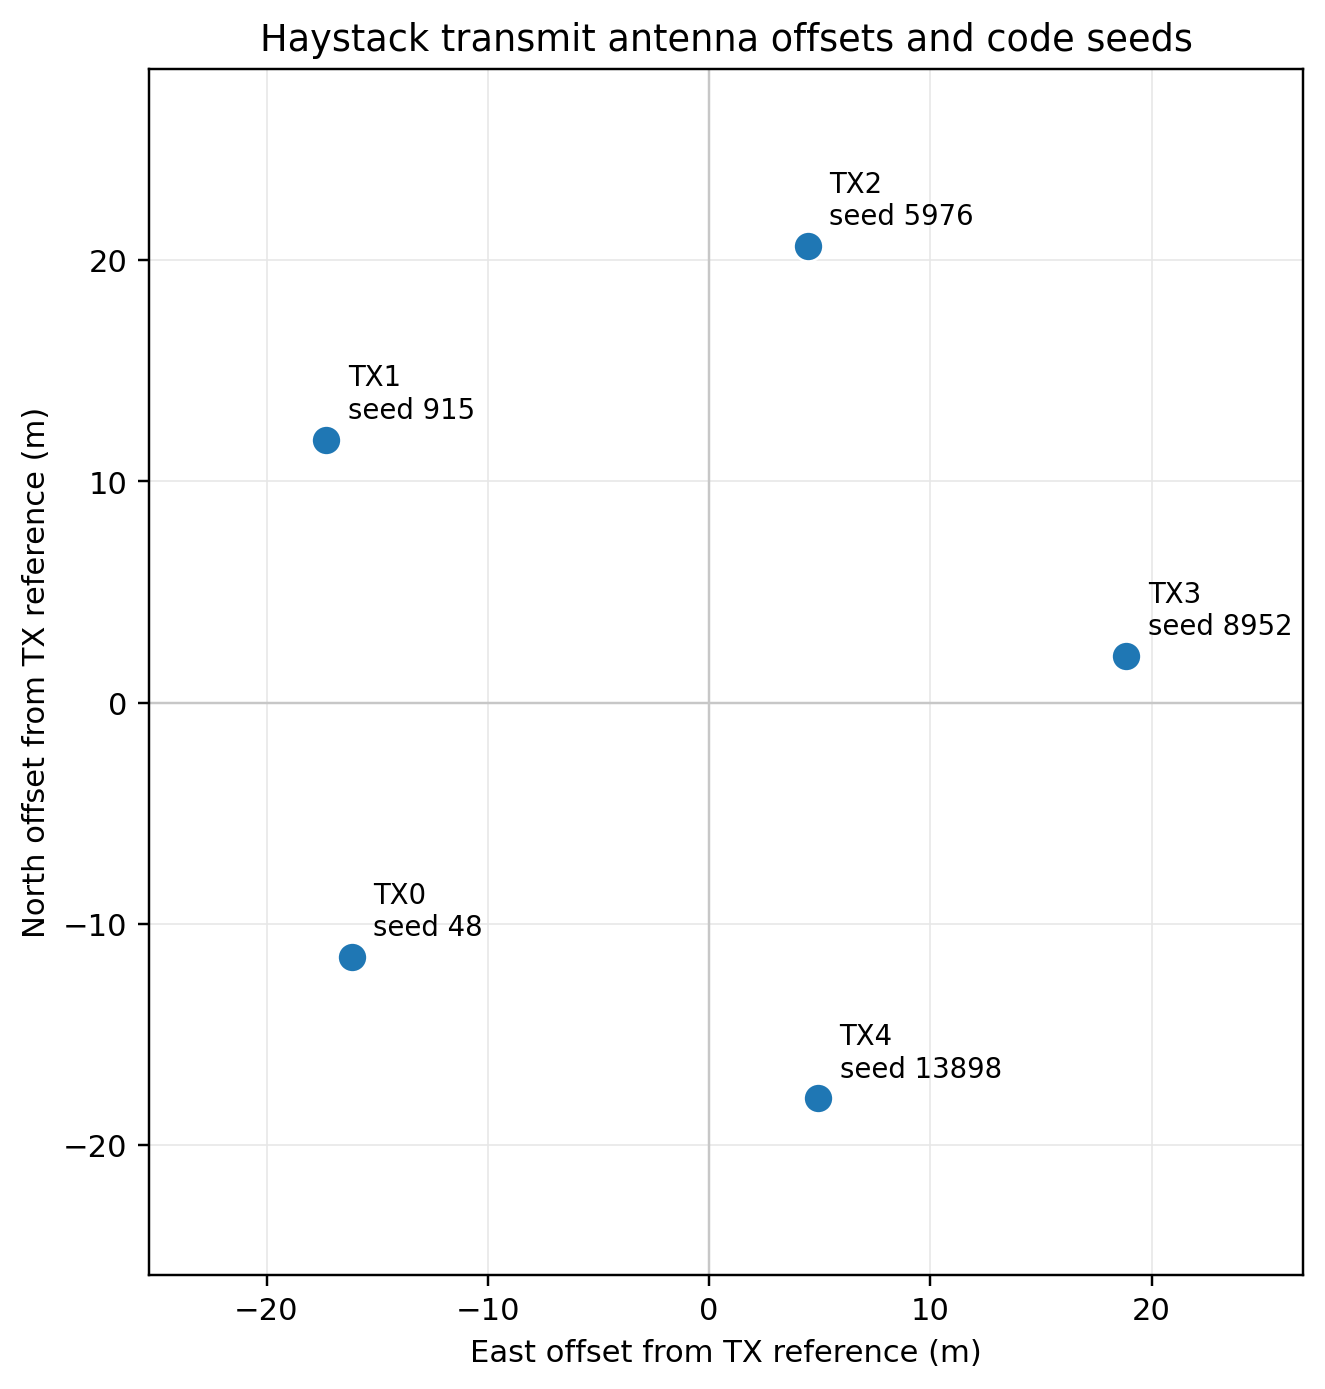
\includegraphics[width=0.72\linewidth]{figures/tx_antenna_coordinates.png}
  \caption{Haystack transmit antenna ENU offsets and the corresponding
  pseudo-random code seeds from the YAML metadata.  The offsets are relative
  to the transmitter reference point used in the station metadata.}
  \figsource{reports/generate_station_config_assets.py}
  \label{fig:tx-antennas}
\end{figure}

The high-resolution products span 18:06:15--18:06:25 UTC.  Two range--time
products are formed.  The first retains the strongest Doppler bin at each
range and is most useful for non-specular trail echoes.  The second requires
\(|f_D| \ge 250\) Hz before peak selection and is used for head-echo trajectory
determination.  Instrumental details and processing checks not needed for the
main interpretation are given in the appendices.

\section{Methods}

\subsection{Range--Doppler Matched Filtering}

Complex voltage samples were corrected for receiver DC offsets before matched
filtering by subtracting one complex mean voltage from each channel over the
read interval.  The same complex-mean DC subtraction was applied to both raw
receiver polarization streams before any polarization combination or
range--Doppler matched filtering.

For each receiver station, channel, transmit code, range gate, and time step,
a window of complex voltage data was multiplied by the conjugate of the
repeated transmit code.  A Fourier transform along the coherent integration
window then produced the Doppler spectrum.  The Doppler FFT was zero padded to
four times the eight-code coherent integration length, increasing the sampled
Doppler-bin density while leaving the coherent integration time unchanged.
Power was averaged incoherently over the two receiver channels and all transmit
codes:
\[
  S(r,f) =
  \frac{1}{N_{\mathrm{ch}}N_{\mathrm{tx}}}
  \sum_{c=1}^{N_{\mathrm{ch}}}
  \sum_{m=1}^{N_{\mathrm{tx}}}
  \left|Z_{c,m}(r,f)\right|^2 .
\]
The range--time product stores the selected peak power \(P(t,r)\), the
selected Doppler \(D(t,r)\), and a noise estimate \(N(t,r)\).  The complex
matched-filter output at the selected Doppler bin is also retained for each
receiver channel and transmit code as
\texttt{voltage\_peak[t, channel, range, tx\_code]}, allowing later
interferometric AoD analysis without rerunning the matched filter bank.

Doppler whitening was applied before peak selection by normalizing each
Doppler bin by its median power over range.  This operation reduces
Doppler-dependent clutter and background structure.  The head-echo
measurements used for trajectory determination were selected from the
Doppler-gated range--time products, while near-zero-Doppler selections were
used to identify non-specular trail echoes.

\subsection{Transmit Interferometric Angle of Departure}

Classical specular meteor radars estimate an angle of arrival (AoA) with a
single transmitter and a receive interferometer, most commonly a five-antenna
Jones-type configuration \cite{jones_1998_interferometer,hocking_2001_realtime,
holdsworth_2004_buckland,holdsworth_2005_allsky}.  The Haystack
configuration used here moves the interferometer to the transmitting side: the
five collocated transmit antennas radiate mutually distinguishable
pseudorandom coded-CW waveforms on the same carrier.  After matched-filter
decoding, one receiver channel contains five code-separated complex voltages,
so each receiver forms a multiple-input/single-output coded-CW meteor radar
(MISO-CW).  Considering the two receiver polarizations and all receiving sites
together gives a multiple-input/multiple-output (MIMO) data set.  This is the
same architecture described by \textcite{chau_2019_mimo}, in which transmit
interferometry gives the angle of departure (AoD) of an echo with respect to
the transmitter, while a conventional receive interferometer gives AoA with
respect to the receiver.  The waveform-diversity idea is standard in MIMO radar
\cite{fishler_2004_mimo,li_stoica_2007_mimo,haimovich_2008_mimo}, and coded-CW
meteor radars exploit the same separation of simultaneous transmitters using
orthogonal or low-cross-correlation codes \cite{vierinen_2016_mimo,
chau_2019_mimo,chau_2021_peru}.  Coherent MIMO methods have also been applied
to atmospheric radar imaging outside the meteor problem
\cite{urco_2018_coherent_mimo,urco_2019_maarsy}.  The practical advantage for
the Cape Cod Bay bolide is that the matched-filter products retain a complex
voltage for each transmit element at a common bistatic range and Doppler bin,
allowing transmit-side interferometric checks without requiring a receive
antenna array at every remote station.

The interferometric phase model follows the spatial-coherence formulation of
\textcite{chau_2019_mimo}.  For a far-field target viewed from the transmitter
array, the phase difference between transmitters \(p\) and \(q\) is
\[
  \rho_{pq} \propto
  \exp\left[-i{\bf k}_T\cdot({\bf r}_p-{\bf r}_q)
             + i\Delta\phi_{pq}\right],
\]
where \({\bf k}_T=(2\pi/\lambda){\bf \hat u}\) points along the transmitter
AoD, \({\bf r}_p-{\bf r}_q\) is the transmitter baseline, and
\(\Delta\phi_{pq}\) is the instrumental phase offset for the pair.  This is
the transmit-side analogue of the receive-interferometer AoA equation.  The
far-field approximation is excellent here because the Haystack transmit
baselines are much smaller than the approximately 200--500 km echo ranges.
Instrumental phase calibration is nevertheless part of the general problem;
meteor-radar phase calibration and complex-plane angle estimation are discussed
by \textcite{holdsworth_2004_phase,chau_clahsen_2019_phase,
vaudrin_2018_complex,younger_reid_2017_precalculated}.  In this first bolide
analysis, AoD is used as a diagnostic and consistency constraint rather than as
the primary trajectory observable.

For a trial departure unit vector \({\bf \hat u}\) in the transmitter ENU
frame, the transmit steering vector is
\[
  a_m({\bf \hat u}) =
  \exp\left(i\frac{2\pi}{\lambda}{\bf r}_m\cdot{\bf \hat u}\right),
\]
where \({\bf r}_m\) is the ENU position of transmit antenna \(m\) relative to
the array reference point, with any instrumental phase correction omitted from
the present diagnostic.  If \({\bf z}\) is the vector of complex code-separated
matched-filter voltages for one receiver channel, the beamformed AoD match
statistic used for diagnostic plotting is
\[
  B({\bf \hat u}) =
  \frac{\left|{\bf a}({\bf \hat u})^\dagger{\bf z}\right|^2}
       {\|{\bf a}({\bf \hat u})\|^2\|{\bf z}\|^2}.
\]
The same steering convention is used in the AoD plus bistatic-delay position
solutions shown later in the report.  In practice, the finite five-element
aperture produces sidelobes and angular ambiguities, so AoD solutions are
interpreted together with the bistatic range constraint, the head-echo
trajectory, and station-to-station consistency.  The point-spread function in
Fig.~\ref{fig:tx-aod-match} therefore shows the deterministic angular ambiguity
structure of the transmitting array.  It is not itself the complete
measurement covariance: as emphasized for meteor-radar AoA/AoD estimation by
\textcite{chau_2019_mimo} and \textcite{vaudrin_2018_complex}, the statistical
uncertainty also depends on SNR, echo duration, zenith angle/elevation
geometry, and calibration errors.

\begin{figure}
  \centering
  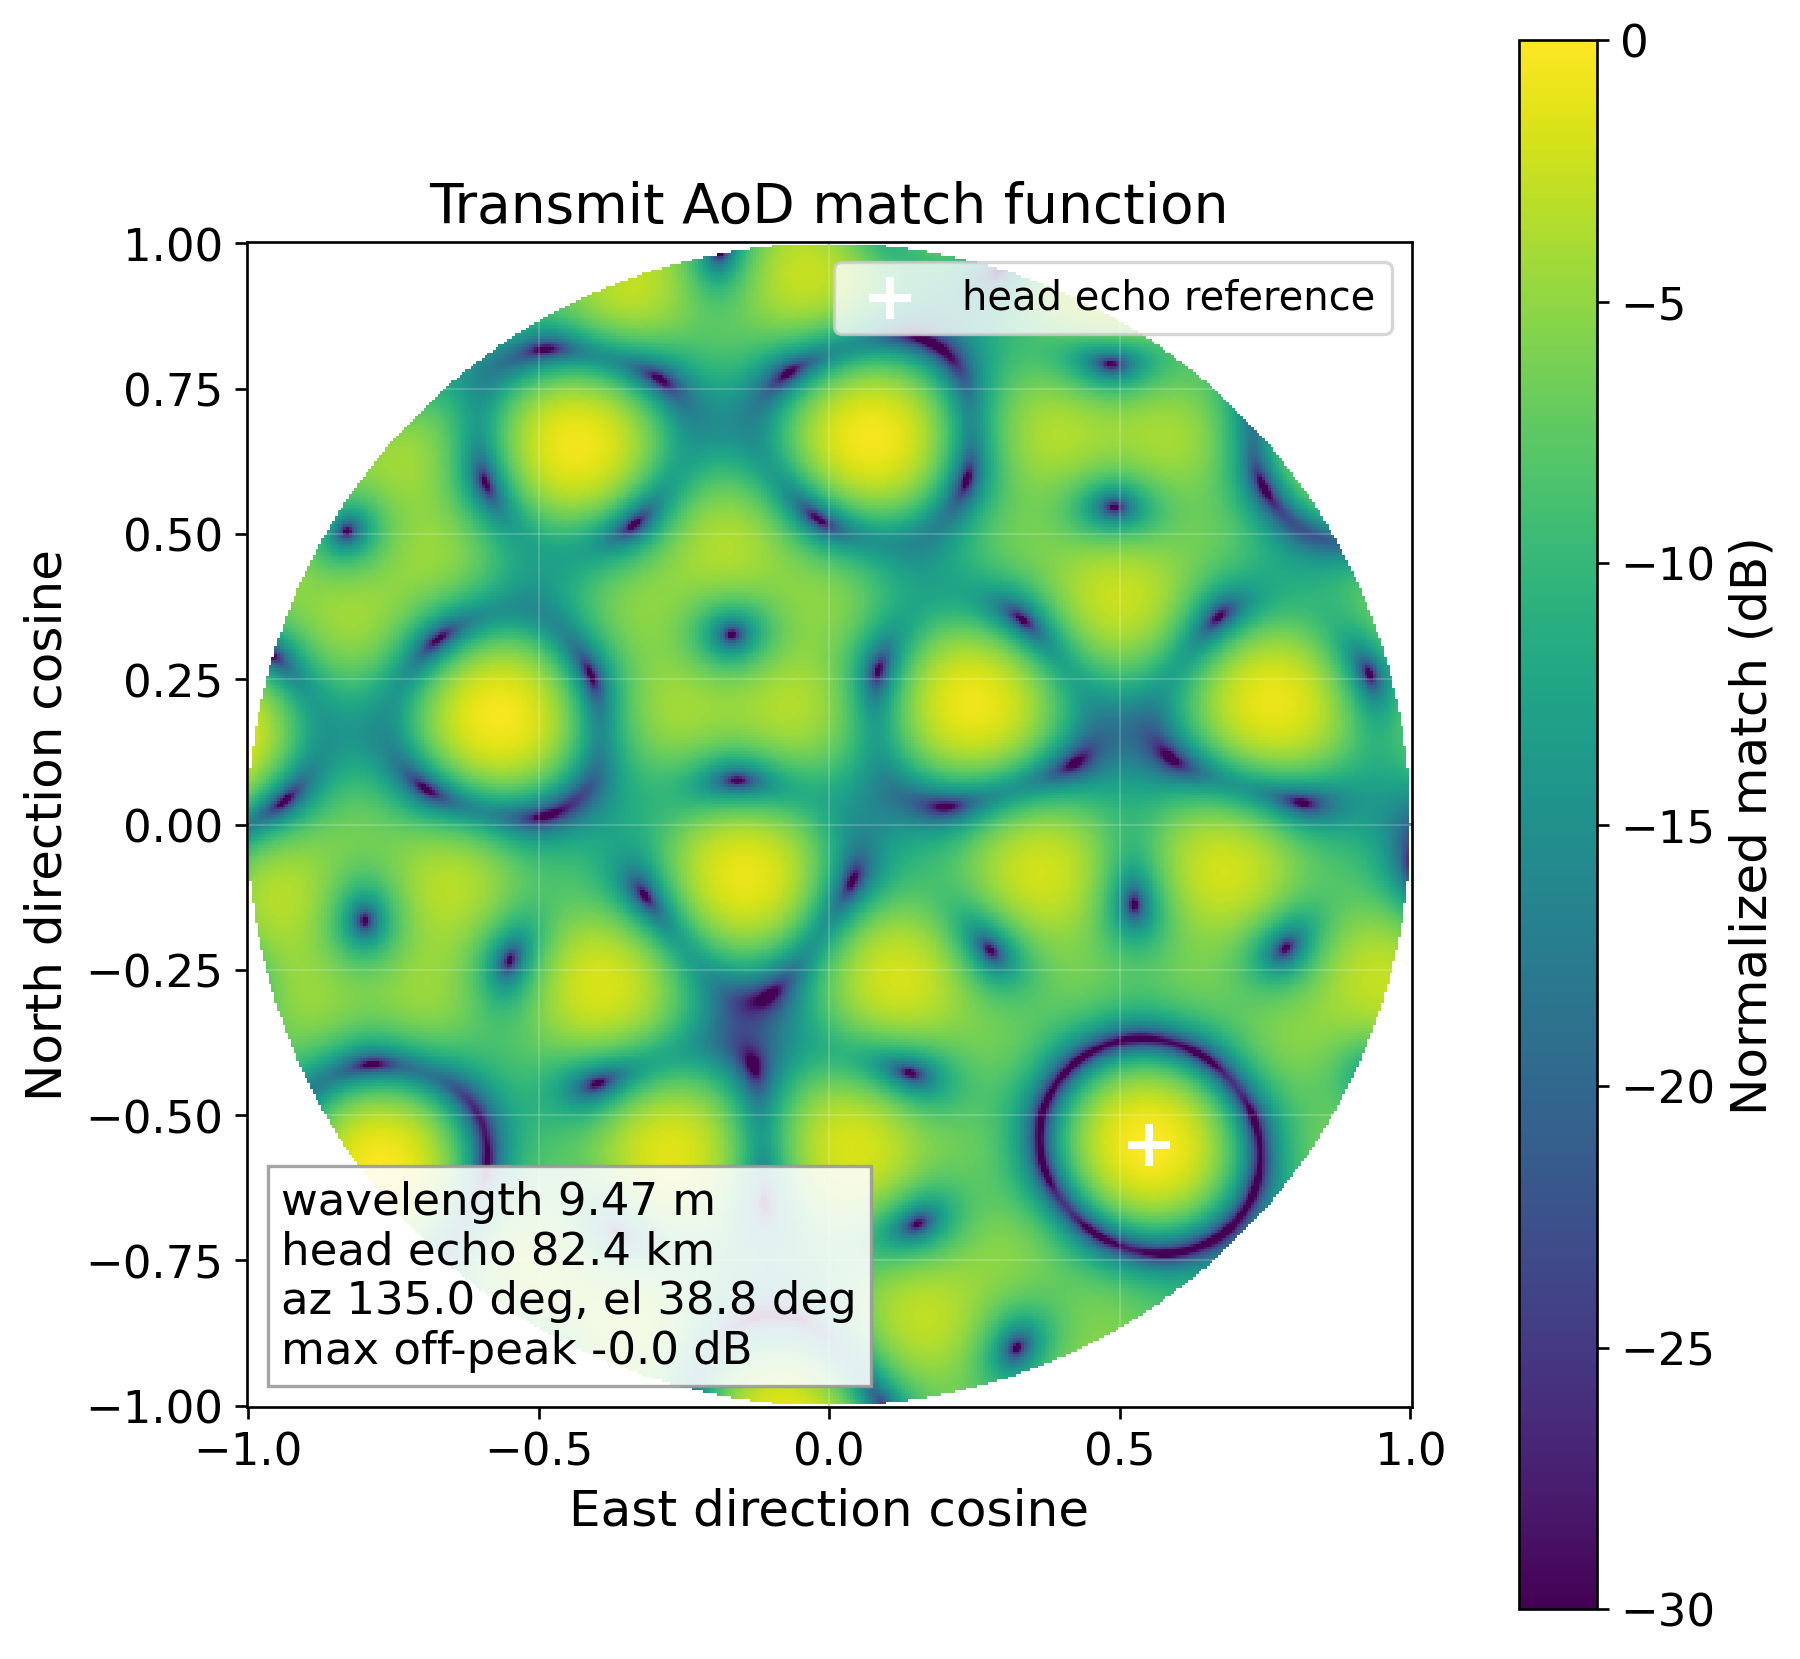
\includegraphics[width=0.78\linewidth]{figures/tx_aod_match_function.png}
  \caption{Transmit-interferometer angle-of-departure point-spread function.
  The plotted quantity is the normalized five-antenna array match function in
  east/north direction cosines over the visible hemisphere.  The reference
  direction is the nominal azimuth and elevation of the tri-static head-echo
  fit at the trajectory reference time, corresponding to an echo altitude of
  82.4 km.  This figure shows the angular response and sidelobe/ambiguity
  structure expected before measurement noise and echo SNR are considered.}
  \figsource{reports/generate_station_config_assets.py}
  \label{fig:tx-aod-match}
\end{figure}

\section{Results}

\subsection{Range--Time Radar Detections}

\begin{figure}
  \centering
  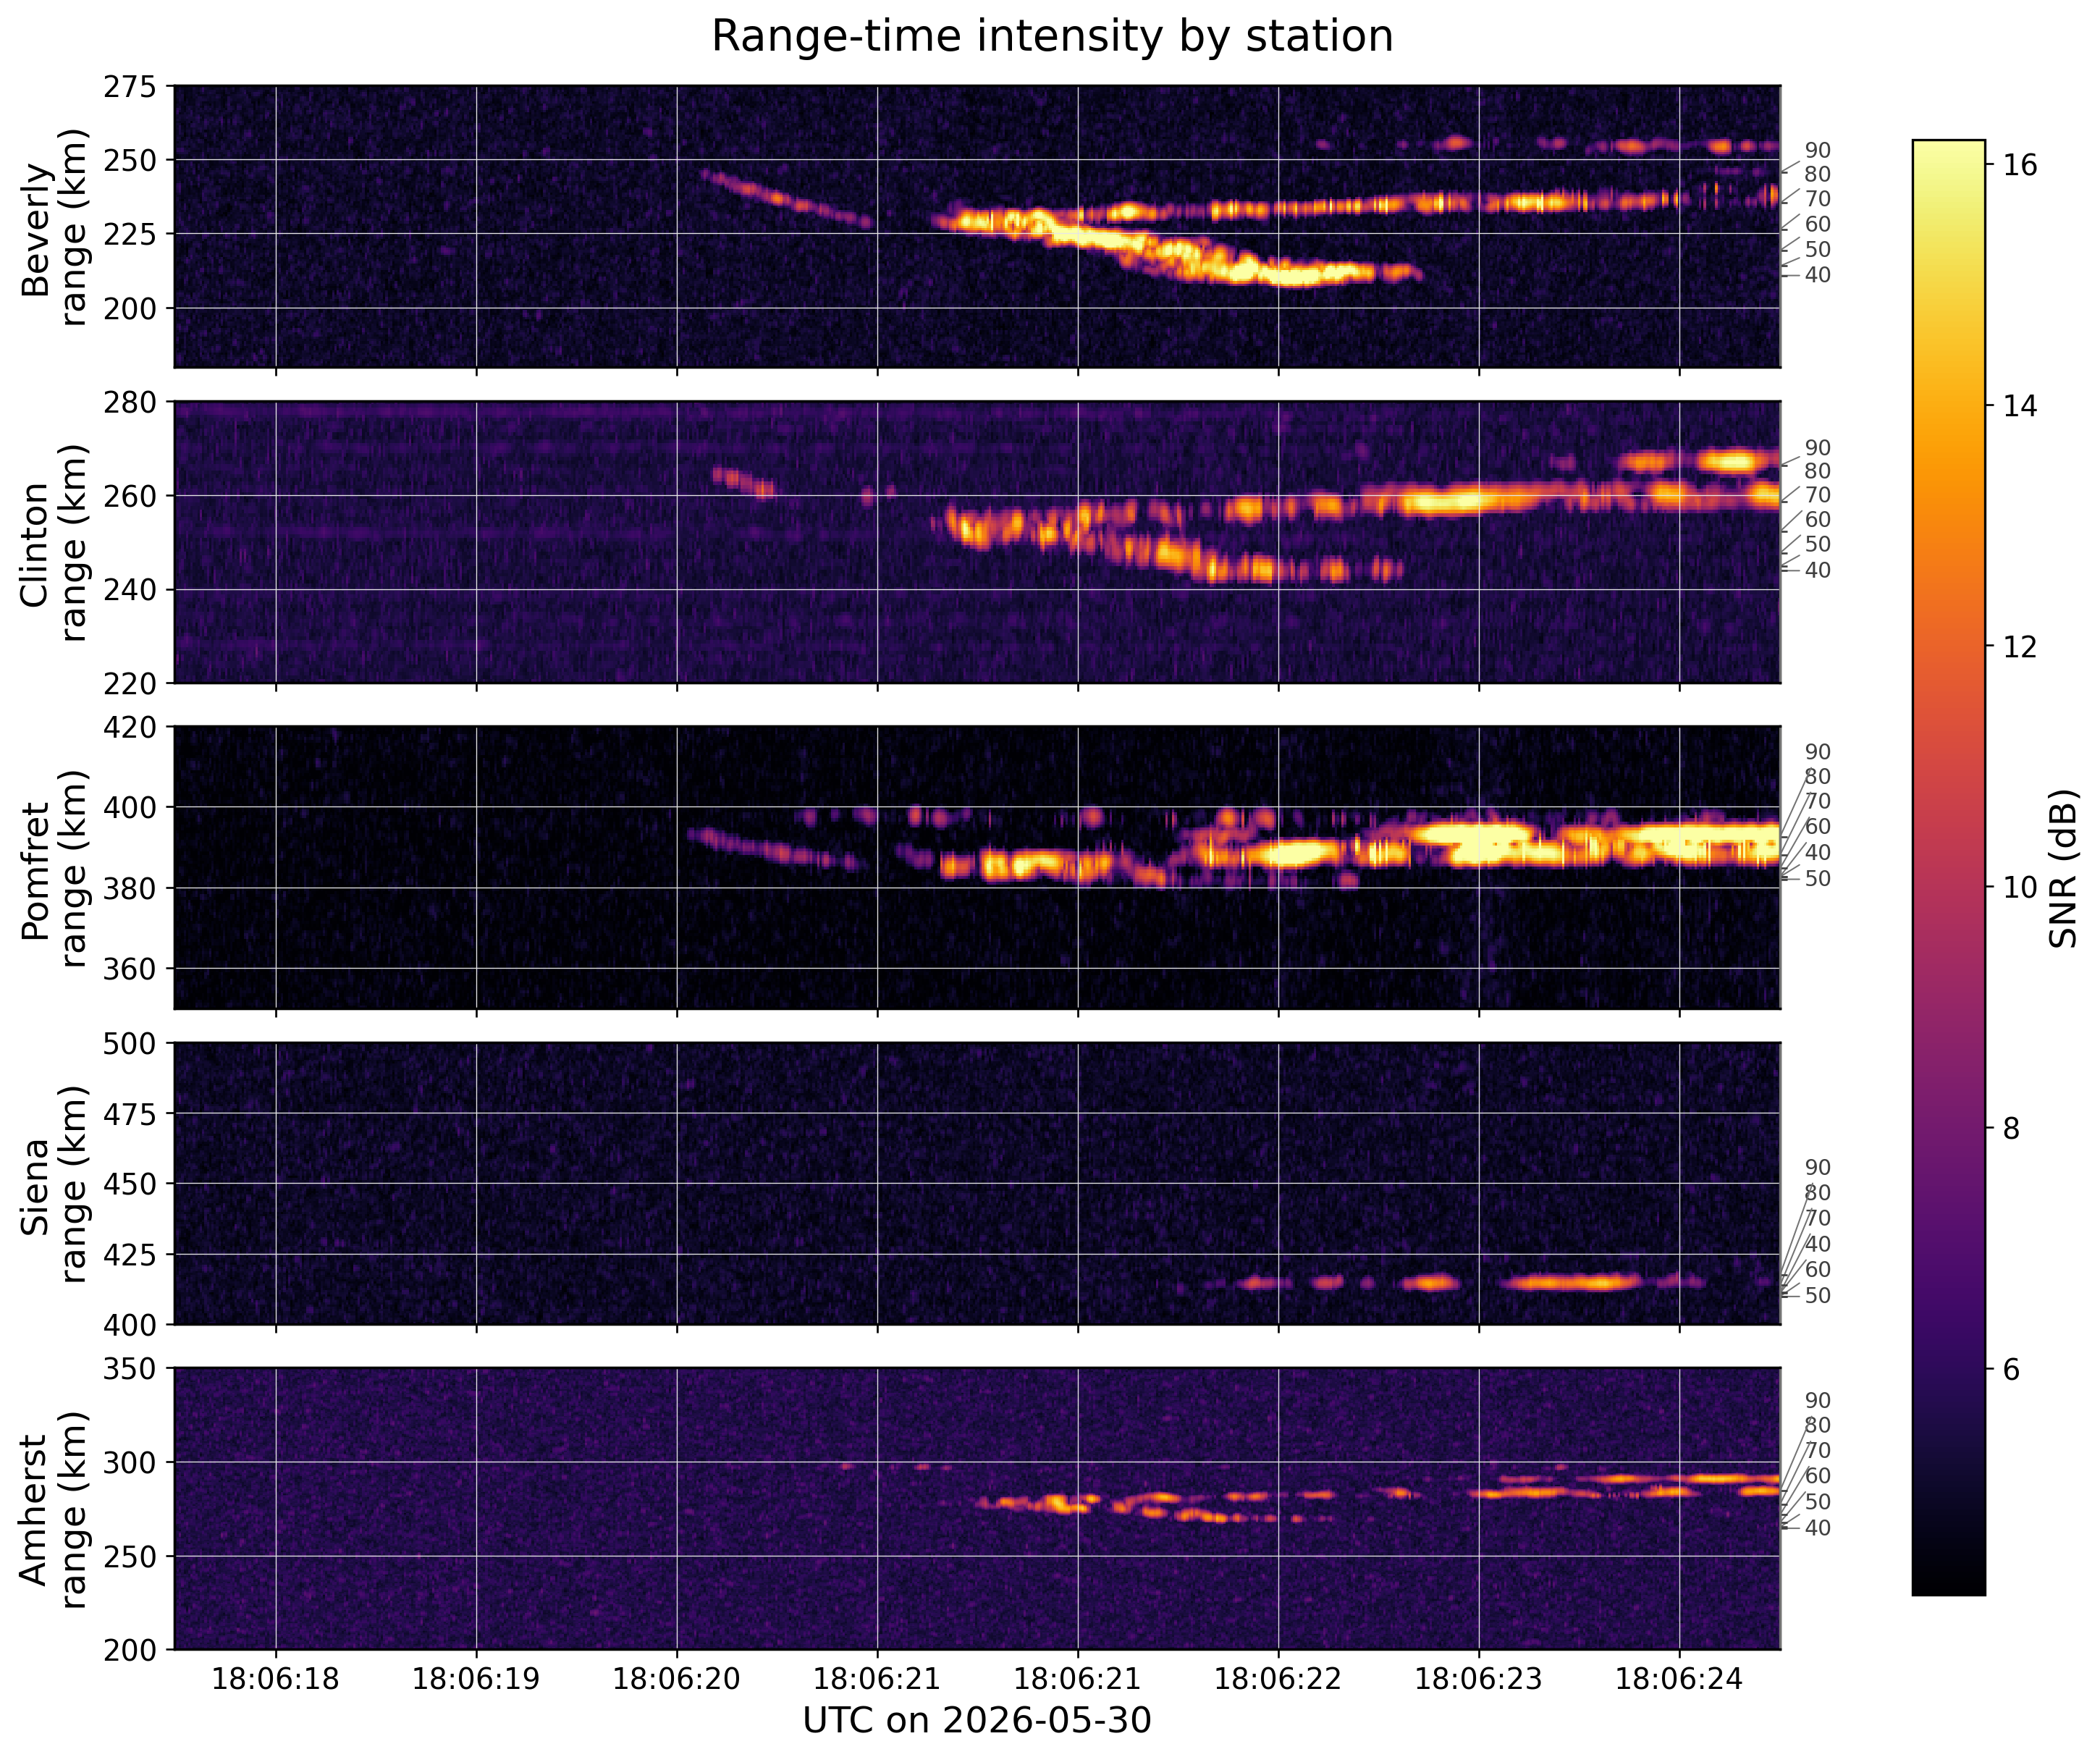
\includegraphics[width=\linewidth]{figures/station_range_time_snr.png}
  \caption{Range--time intensity for all five stations over the
  high-resolution 18:06:18--18:06:25 UTC interval.  The plotted range windows
  are Beverly 180--275 km, Clinton 220--280 km, Pomfret 350--420 km, Siena
  400--500 km, and Amherst 200--350 km.  The right-side manual labels mark the
  meteor altitude inferred from the fitted head-echo trajectory at the
  corresponding bistatic range for each station.}
  \figsource{reports/generate_station_rti_figures.py}
  \label{fig:station-rti-snr}
\end{figure}

\begin{figure}
  \centering
  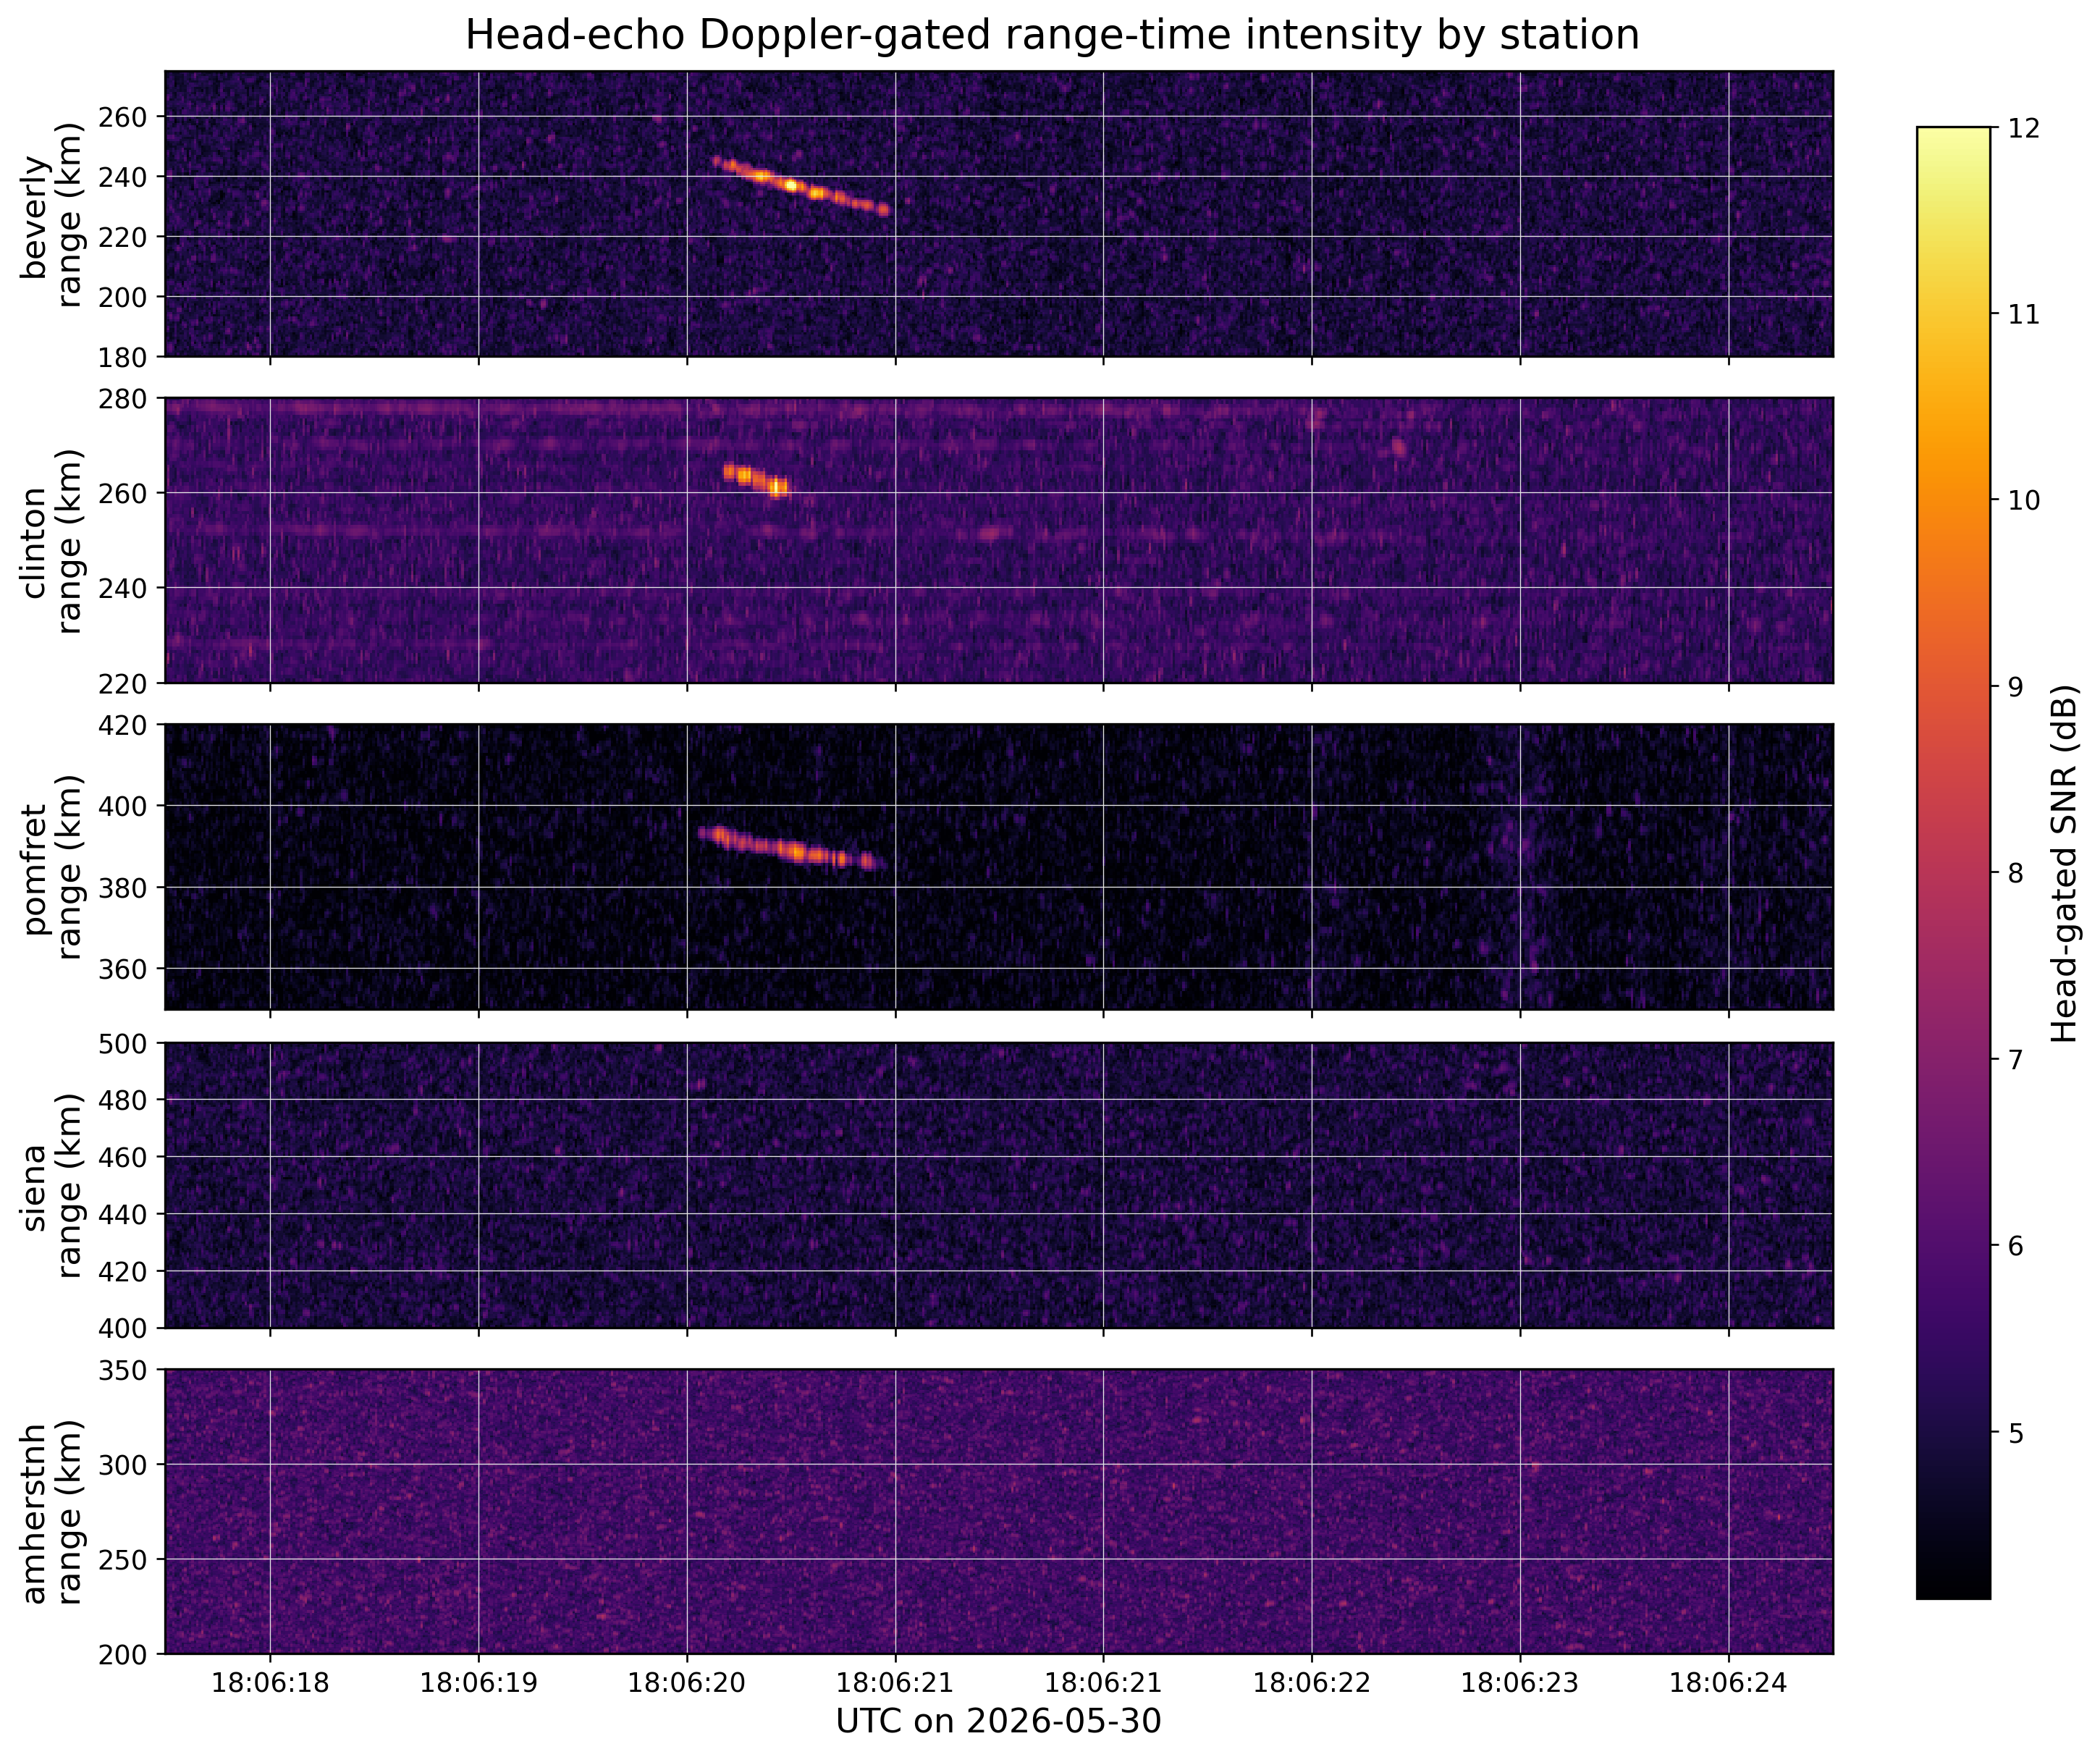
\includegraphics[width=\linewidth]{figures/station_range_time_head_snr.png}
  \caption{Range--time SNR from 18:06:19 to 18:06:22 UTC over the same
  station range windows as Figure~\ref{fig:station-rti-snr}, but using the
  meteor head-echo Doppler selection criterion.  At each time and range gate,
  the plotted SNR is the peak selected after requiring \(|f_D| \ge 250\) Hz,
  suppressing the near-zero-Doppler trail/clutter bins emphasized in the
  all-Doppler RTI.}
  \figsource{reports/generate_station_rti_figures.py}
  \label{fig:station-rti-head-snr}
\end{figure}

\begin{figure}
  \centering
  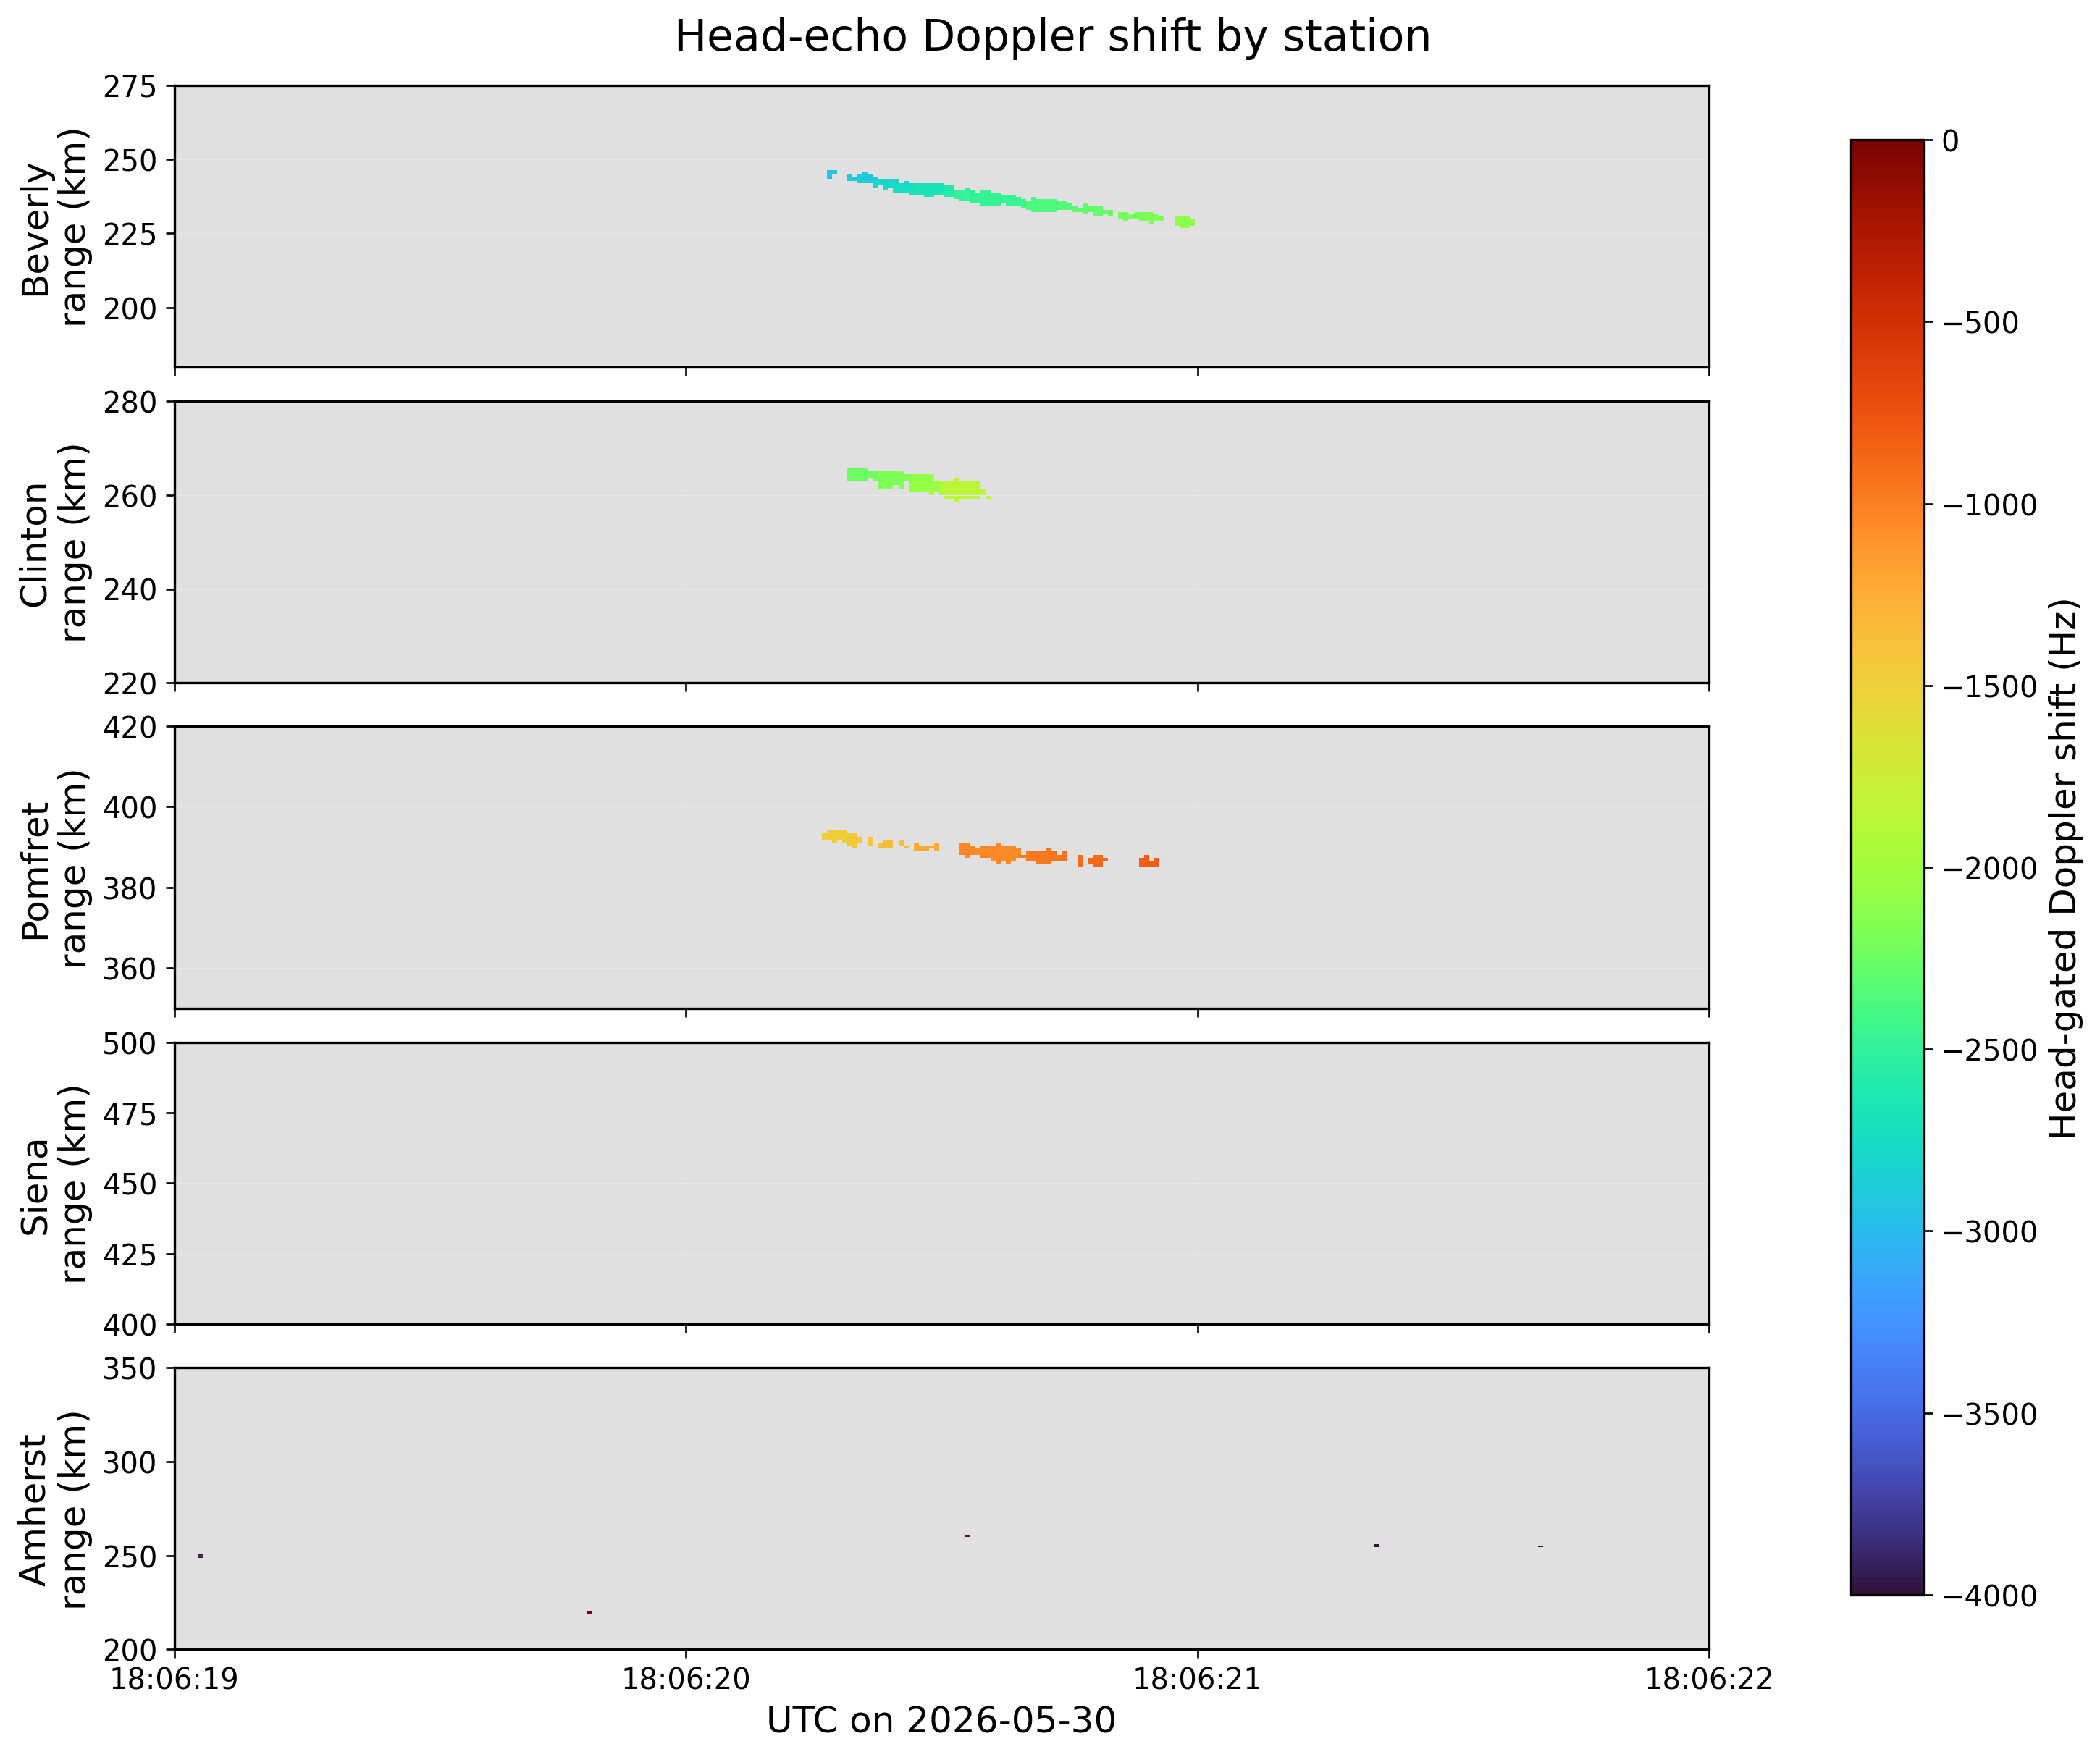
\includegraphics[width=\linewidth]{figures/station_range_time_head_doppler.png}
  \caption{Doppler shift from 18:06:19 to 18:06:22 UTC for the same
  head-echo-selected bins shown in Figure~\ref{fig:station-rti-head-snr}.
  Values are shown only where the head-gated SNR is at least 7.5 dB.}
  \figsource{reports/generate_station_rti_figures.py}
  \label{fig:station-rti-head-doppler}
\end{figure}

\begin{figure}
  \centering
  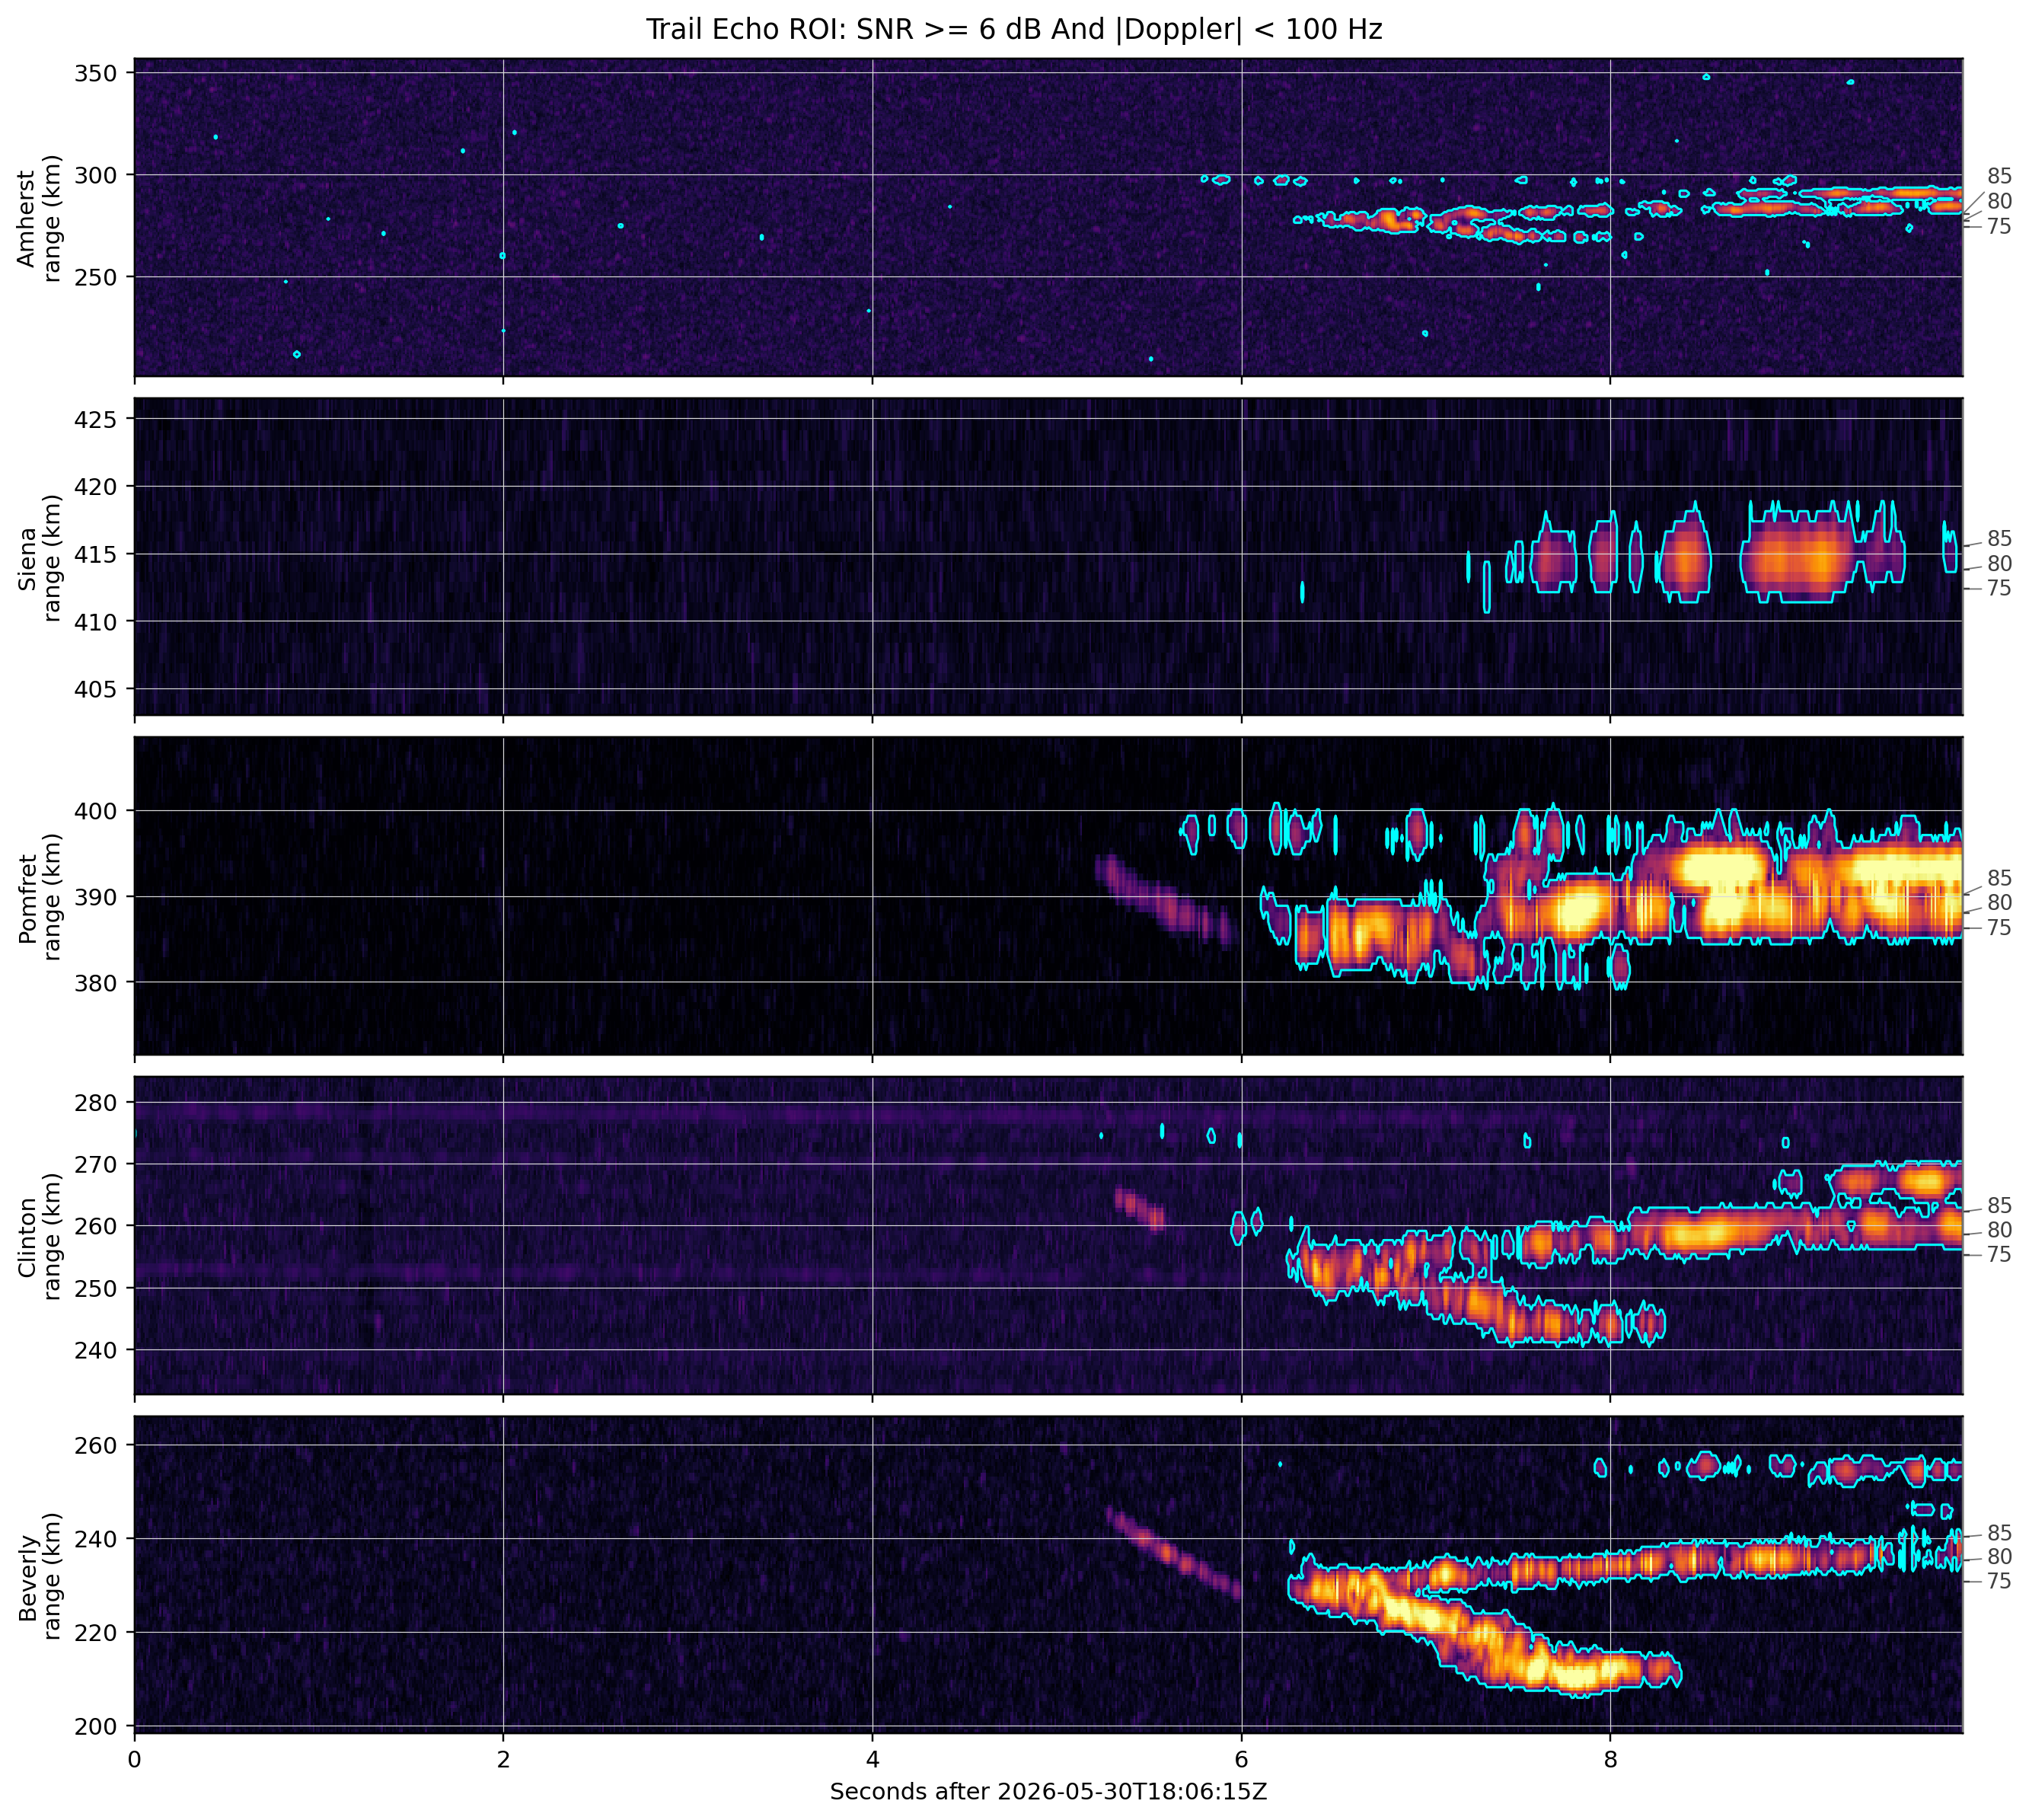
\includegraphics[width=\linewidth]{figures/trail_echo_roi.png}
  \caption{Near-zero-Doppler trail echo ROI for Amherst, Siena, Pomfret,
  Clinton, and Beverly.  The plotted intensity is the all-Doppler range--time
  SNR product used to select near-zero-Doppler trail cells with SNR at least
  6 dB and \(|f_D| < 100\) Hz.  The faint dashed white curves show the
  bistatic range predicted by the head-echo trajectory fit for each station;
  the trajectory is not drawn after the fitted height drops below sea level.
  Height annotations in the top panel mark selected altitudes along the fitted
  trajectory.}
  \figsource{trail_echo_roi.py}
  \label{fig:trail-echo-roi}
\end{figure}

\subsection{Trajectory, Trail Echoes, and Dark Flight}

The head-echo trajectory was determined from manually selected head-echo
regions of interest (ROIs) in the Beverly, Clinton, and Pomfret
range--Doppler products.  Within each station ROI, one measurement was
extracted at each time step by
choosing the range gate with the largest SNR, subject to a minimum SNR of
5 dB.  Robust outlier rejection was then applied independently to each
station's range and Doppler sequence.  The first
\TrajectoryPomfretStartTrimS{} s of Pomfret measurements were excluded because
these earliest picks are inconsistent with the subsequent Pomfret trend.  The
final fit contains \TrajectoryNObservations{} retained measurements and
excludes \TrajectoryNRejected{} ROI peak measurements as outliers or
station-start trimmed points.

The fitted state is a six-parameter straight-line trajectory in the local ENU
frame of the transmitter,
\[
  {\bf x}(t) = {\bf x}_0 + {\bf v}(t-t_0).
\]
with both bistatic range and bistatic Doppler fit simultaneously.  For each
transmitter--meteor--receiver path, the bistatic range model is
\[
  R_b(t)=|{\bf x}(t)-{\bf x}_{\mathrm{tx}}|
             +|{\bf x}(t)-{\bf x}_{\mathrm{rx}}|,
\]
and the bistatic Doppler model is
\[
  f_D(t)=\frac{f_0}{c}
  \left[
    \frac{{\bf x}(t)-{\bf x}_{\mathrm{tx}}}
         {|{\bf x}(t)-{\bf x}_{\mathrm{tx}}|}
    +
    \frac{{\bf x}(t)-{\bf x}_{\mathrm{rx}}}
         {|{\bf x}(t)-{\bf x}_{\mathrm{rx}}|}
  \right]\cdot{\bf v}(t).
\]
The trajectory parameters were estimated by minimizing the weighted
range--Doppler cost function
\[
  \chi^2({\bf p}) =
  \sum_{i=1}^{N}
  \left\{
  \left[
    \frac{R_i^{\mathrm{obs}}-R_b(t_i;{\bf p},s_i)}
         {\sigma_R}
  \right]^2
  +
  \left[
    \frac{f_{D,i}^{\mathrm{obs}}-f_D(t_i;{\bf p},s_i)}
         {\sigma_f}
  \right]^2
  \right\},
\]
where \({\bf p}=({\bf x}_0,{\bf v})\), \(s_i\) denotes the receiver station
for measurement \(i\).  The fixed weights use \(\sigma_R=750\) m for bistatic
range and \(\sigma_f=500\) Hz for Doppler.  The two uncertainty scales are
kept distinct because the range measurements are in metres whereas the Doppler
measurements are in hertz.
With this sign convention, positive Doppler corresponds to an increasing total
bistatic propagation path.
The residual RMS values for the current fit are \TrajectoryRangeRmsM{} m in
bistatic range and \TrajectoryDopplerRmsHz{} Hz in Doppler.
The uncertainty calculation uses the physical range--Doppler Jacobian from the
nonlinear least-squares fit together with the same correlated measurement model
used in the final linear GLS solve.  The matched-filter measurements are formed
from 16 repeated 10 ms codes, so adjacent time samples from the same receiver
station and the same observable share coherent voltage samples.  We therefore
model the measurement covariance as block diagonal by station and observable,
with separate range and Doppler blocks.  Within each block, the correlation
between two measurements separated by \(k\) code periods is
\[
  \rho(k) = \max\left(0,\ 1-\frac{|k|}{16}\right),
\]
and the covariance entries are
\[
  \Sigma^{(R)}_{ij} = \rho(k_{ij})\,\sigma_{R,i}\sigma_{R,j},
  \qquad
  \Sigma^{(f)}_{ij} = \rho(k_{ij})\,\sigma_{f,i}\sigma_{f,j}.
\]
Range and Doppler are kept independent to first order, so cross-observable
blocks are zero.  With this full measurement covariance \(\boldsymbol{\Sigma}\),
the trajectory covariance is the standard linearized GLS covariance
\[
  \widehat{\bf C}_{p} =
  \left({\bf J}^{T}\boldsymbol{\Sigma}^{-1}{\bf J}\right)^{-1},
\]
where \({\bf J}\) is the finite-difference Jacobian of the native range and
Doppler predictions with respect to \({\bf p}\).  No empirical residual scale
factor is applied to broaden the parameter covariance or the plotted uncertainty
bands.
The long pseudorandom phase code separates delay and Doppler in the matched
filter, removing the range--Doppler ambiguity that would otherwise couple the
two observables.  Inspection of the post-fit residuals does not show a large
station-dependent range bias, although the Doppler residuals retain some
time-correlated structure; the coherent-integration overlap model captures the
dominant sampling correlation but is still an approximate stochastic
description of the residual process.
The shaded bands in
Figure~\ref{fig:trajectory-observables} show the trajectory-parameter
uncertainty: Monte Carlo draws from
\(\mathcal{N}({\bf p},\widehat{\bf C}_{p})\) are propagated through the range
and Doppler equations, and the plotted envelope is the central 95\% interval
of the resulting model curves.

\begin{figure}
  \centering
  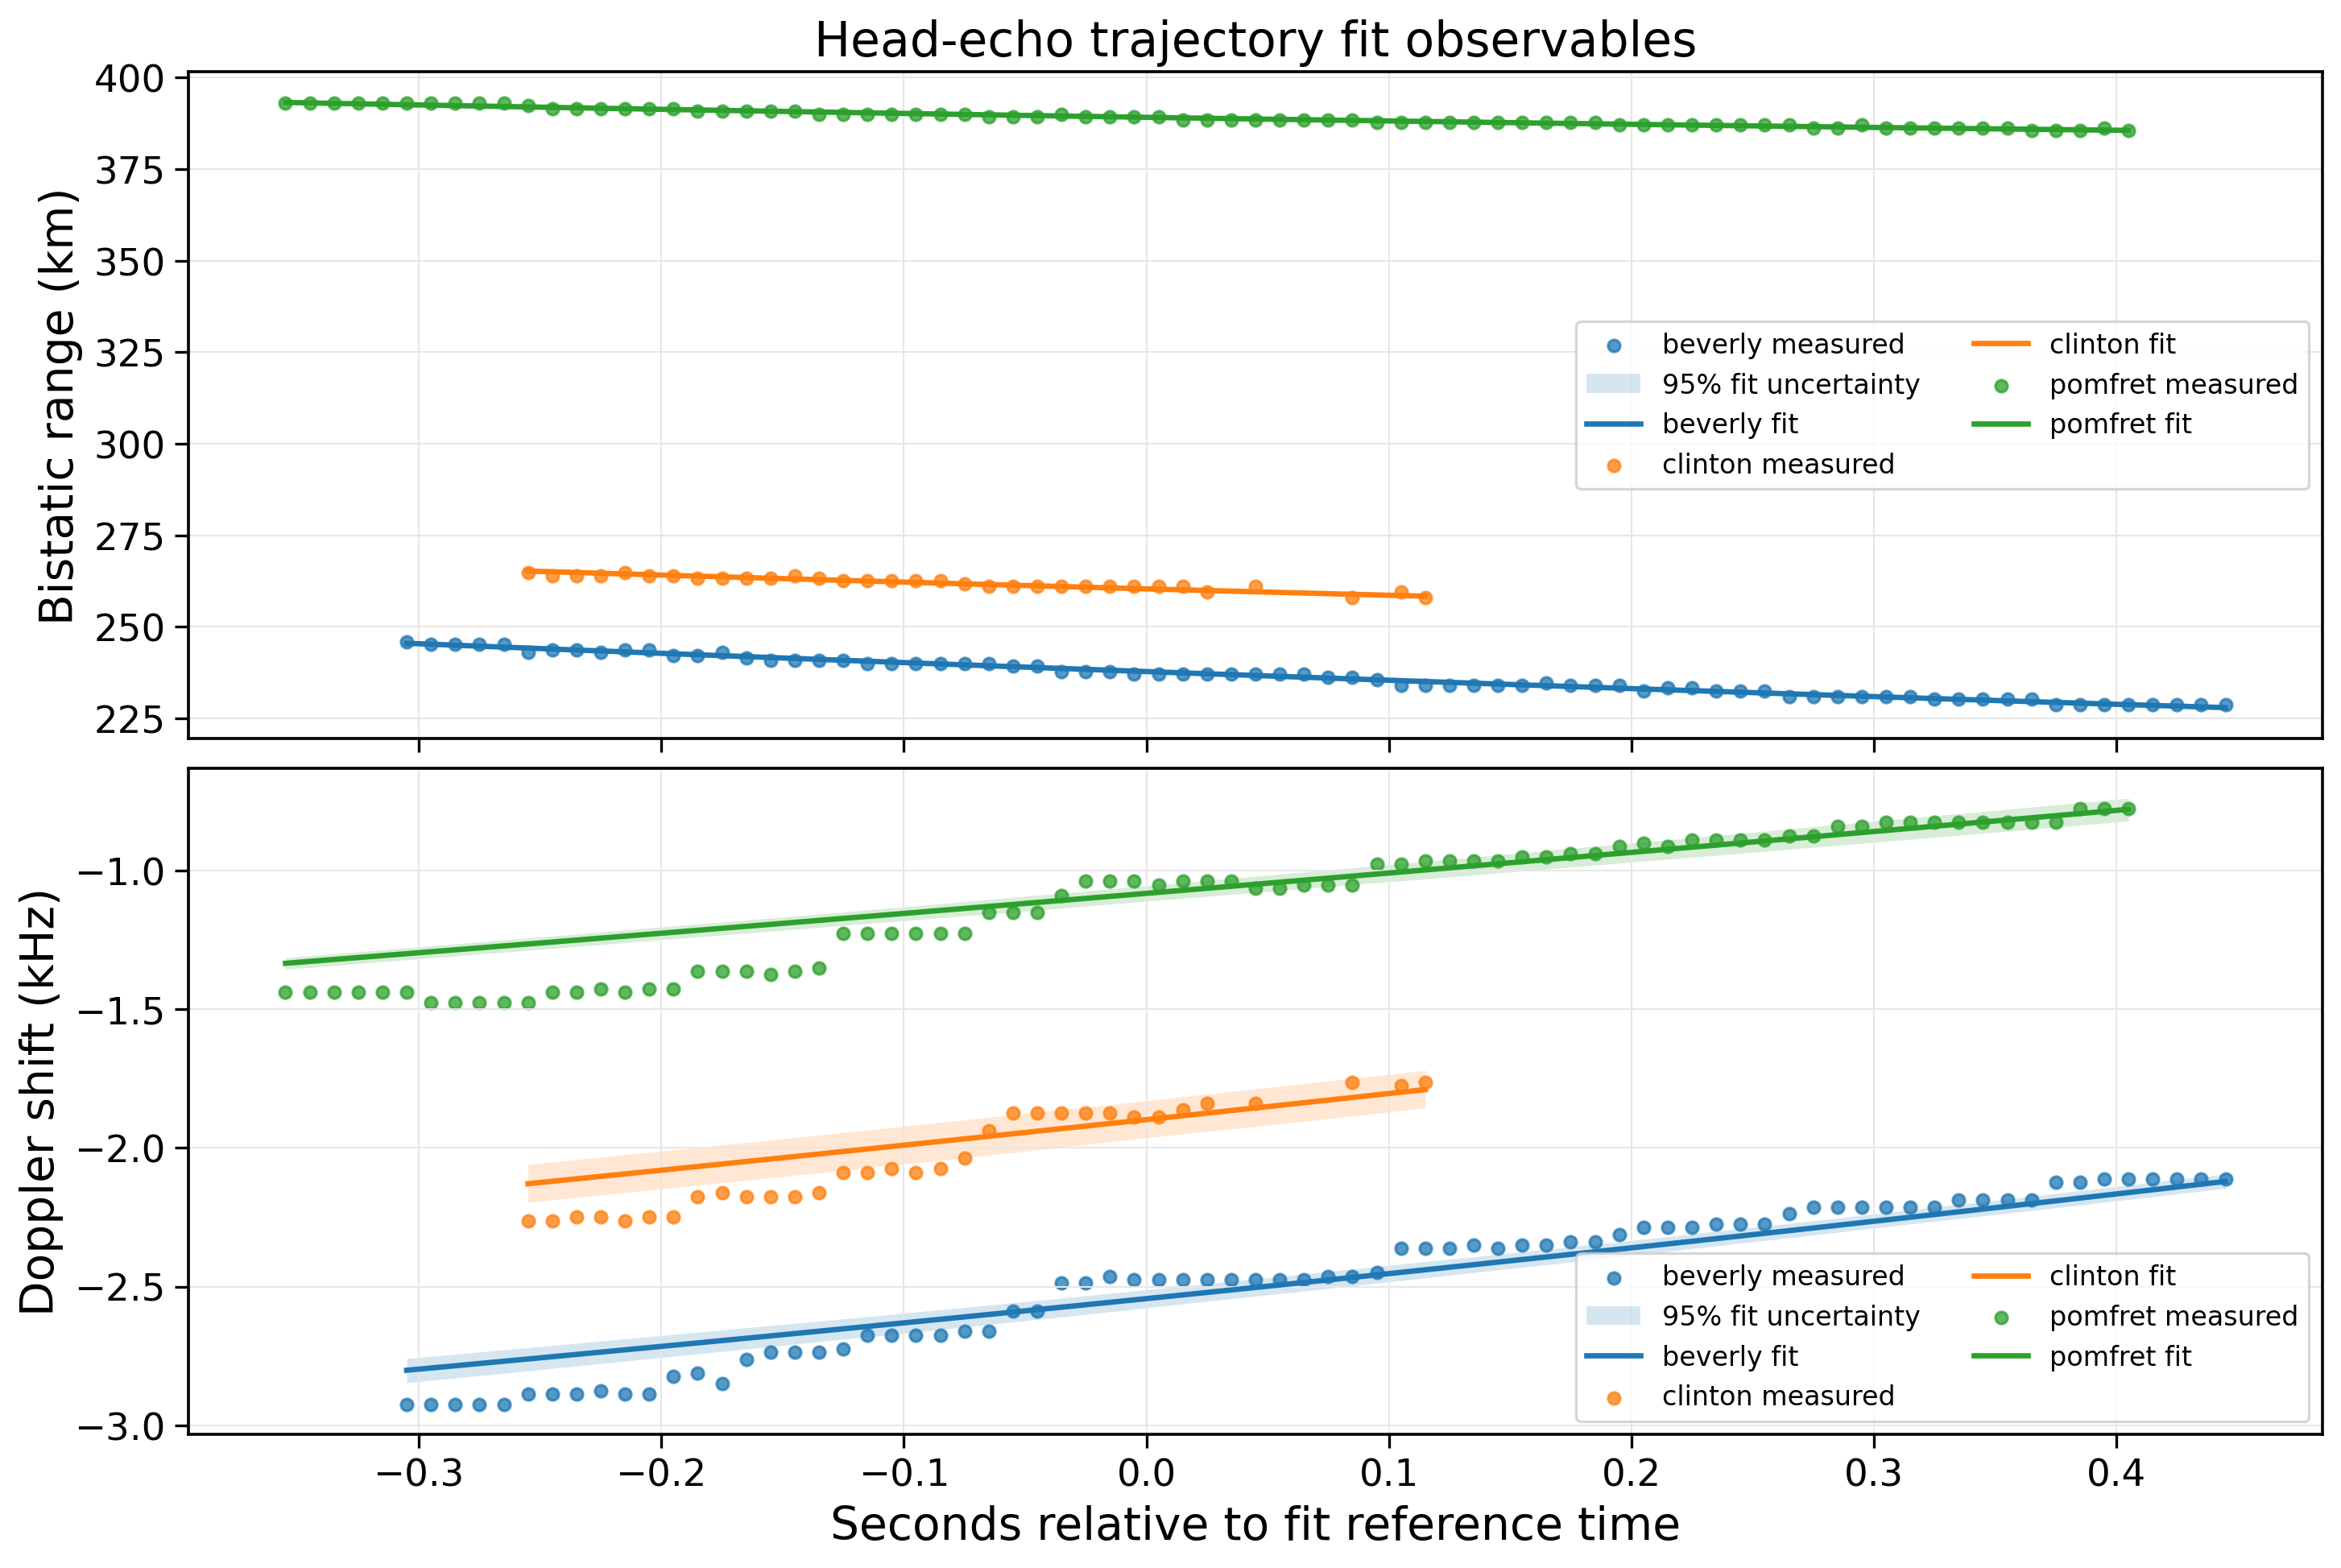
\includegraphics[width=\linewidth]{figures/head_echo_range_doppler_fit.png}
  \caption{Range and Doppler measurements used in the head-echo trajectory
  fit.  Points show the ROI-derived measurements after SNR thresholding and
  outlier rejection; lines show the fitted straight-line trajectory model for
  each bistatic path.  Shaded bands show central 95\% trajectory-parameter
  uncertainty intervals obtained by propagating samples from the correlated
  range--Doppler GLS trajectory covariance through the range and Doppler
  equations.}
  \figsource{reports/generate_trajectory_report_assets.py}
  \label{fig:trajectory-observables}
\end{figure}

The first retained detection occurred at \TrajectoryFirstDetectionUTC{}.  The
best-fit initial detection height was \TrajectoryInitialHeightKm{} km at
latitude \TrajectoryInitialLat{} deg and longitude \TrajectoryInitialLon{} deg.
The fitted initial velocity is
\[
  {\bf v}_{\mathrm{ENU}} =
  (\TrajectoryVEastKmS{},\ \TrajectoryVNorthKmS{},\ \TrajectoryVUpKmS{})
  \ \mathrm{km\,s^{-1}},
\]
with speed \TrajectorySpeedKmS{} km s\(^{-1}\).  The large negative upward
component is consistent with a steeply descending trajectory during the
head-echo interval.  The corresponding apparent radiant, without
zenithal-attraction correction, is RA
\(\TrajectoryRadiantRADeg{}\pm\TrajectoryRadiantRASigmaDeg{}\) deg, Dec
\(\TrajectoryRadiantDecDeg{}\pm\TrajectoryRadiantDecSigmaDeg{}\) deg, or Az
\(\TrajectoryRadiantAzDeg{}\pm\TrajectoryRadiantAzSigmaDeg{}\) deg, El
\(\TrajectoryRadiantElDeg{}\pm\TrajectoryRadiantElSigmaDeg{}\) deg in the
local horizon frame at the first detection point.  The quoted speed
uncertainty is \(\TrajectorySpeedSigmaKmS{}\) km s\(^{-1}\), computed from the
same covariance samples.

\begin{figure}
  \centering
  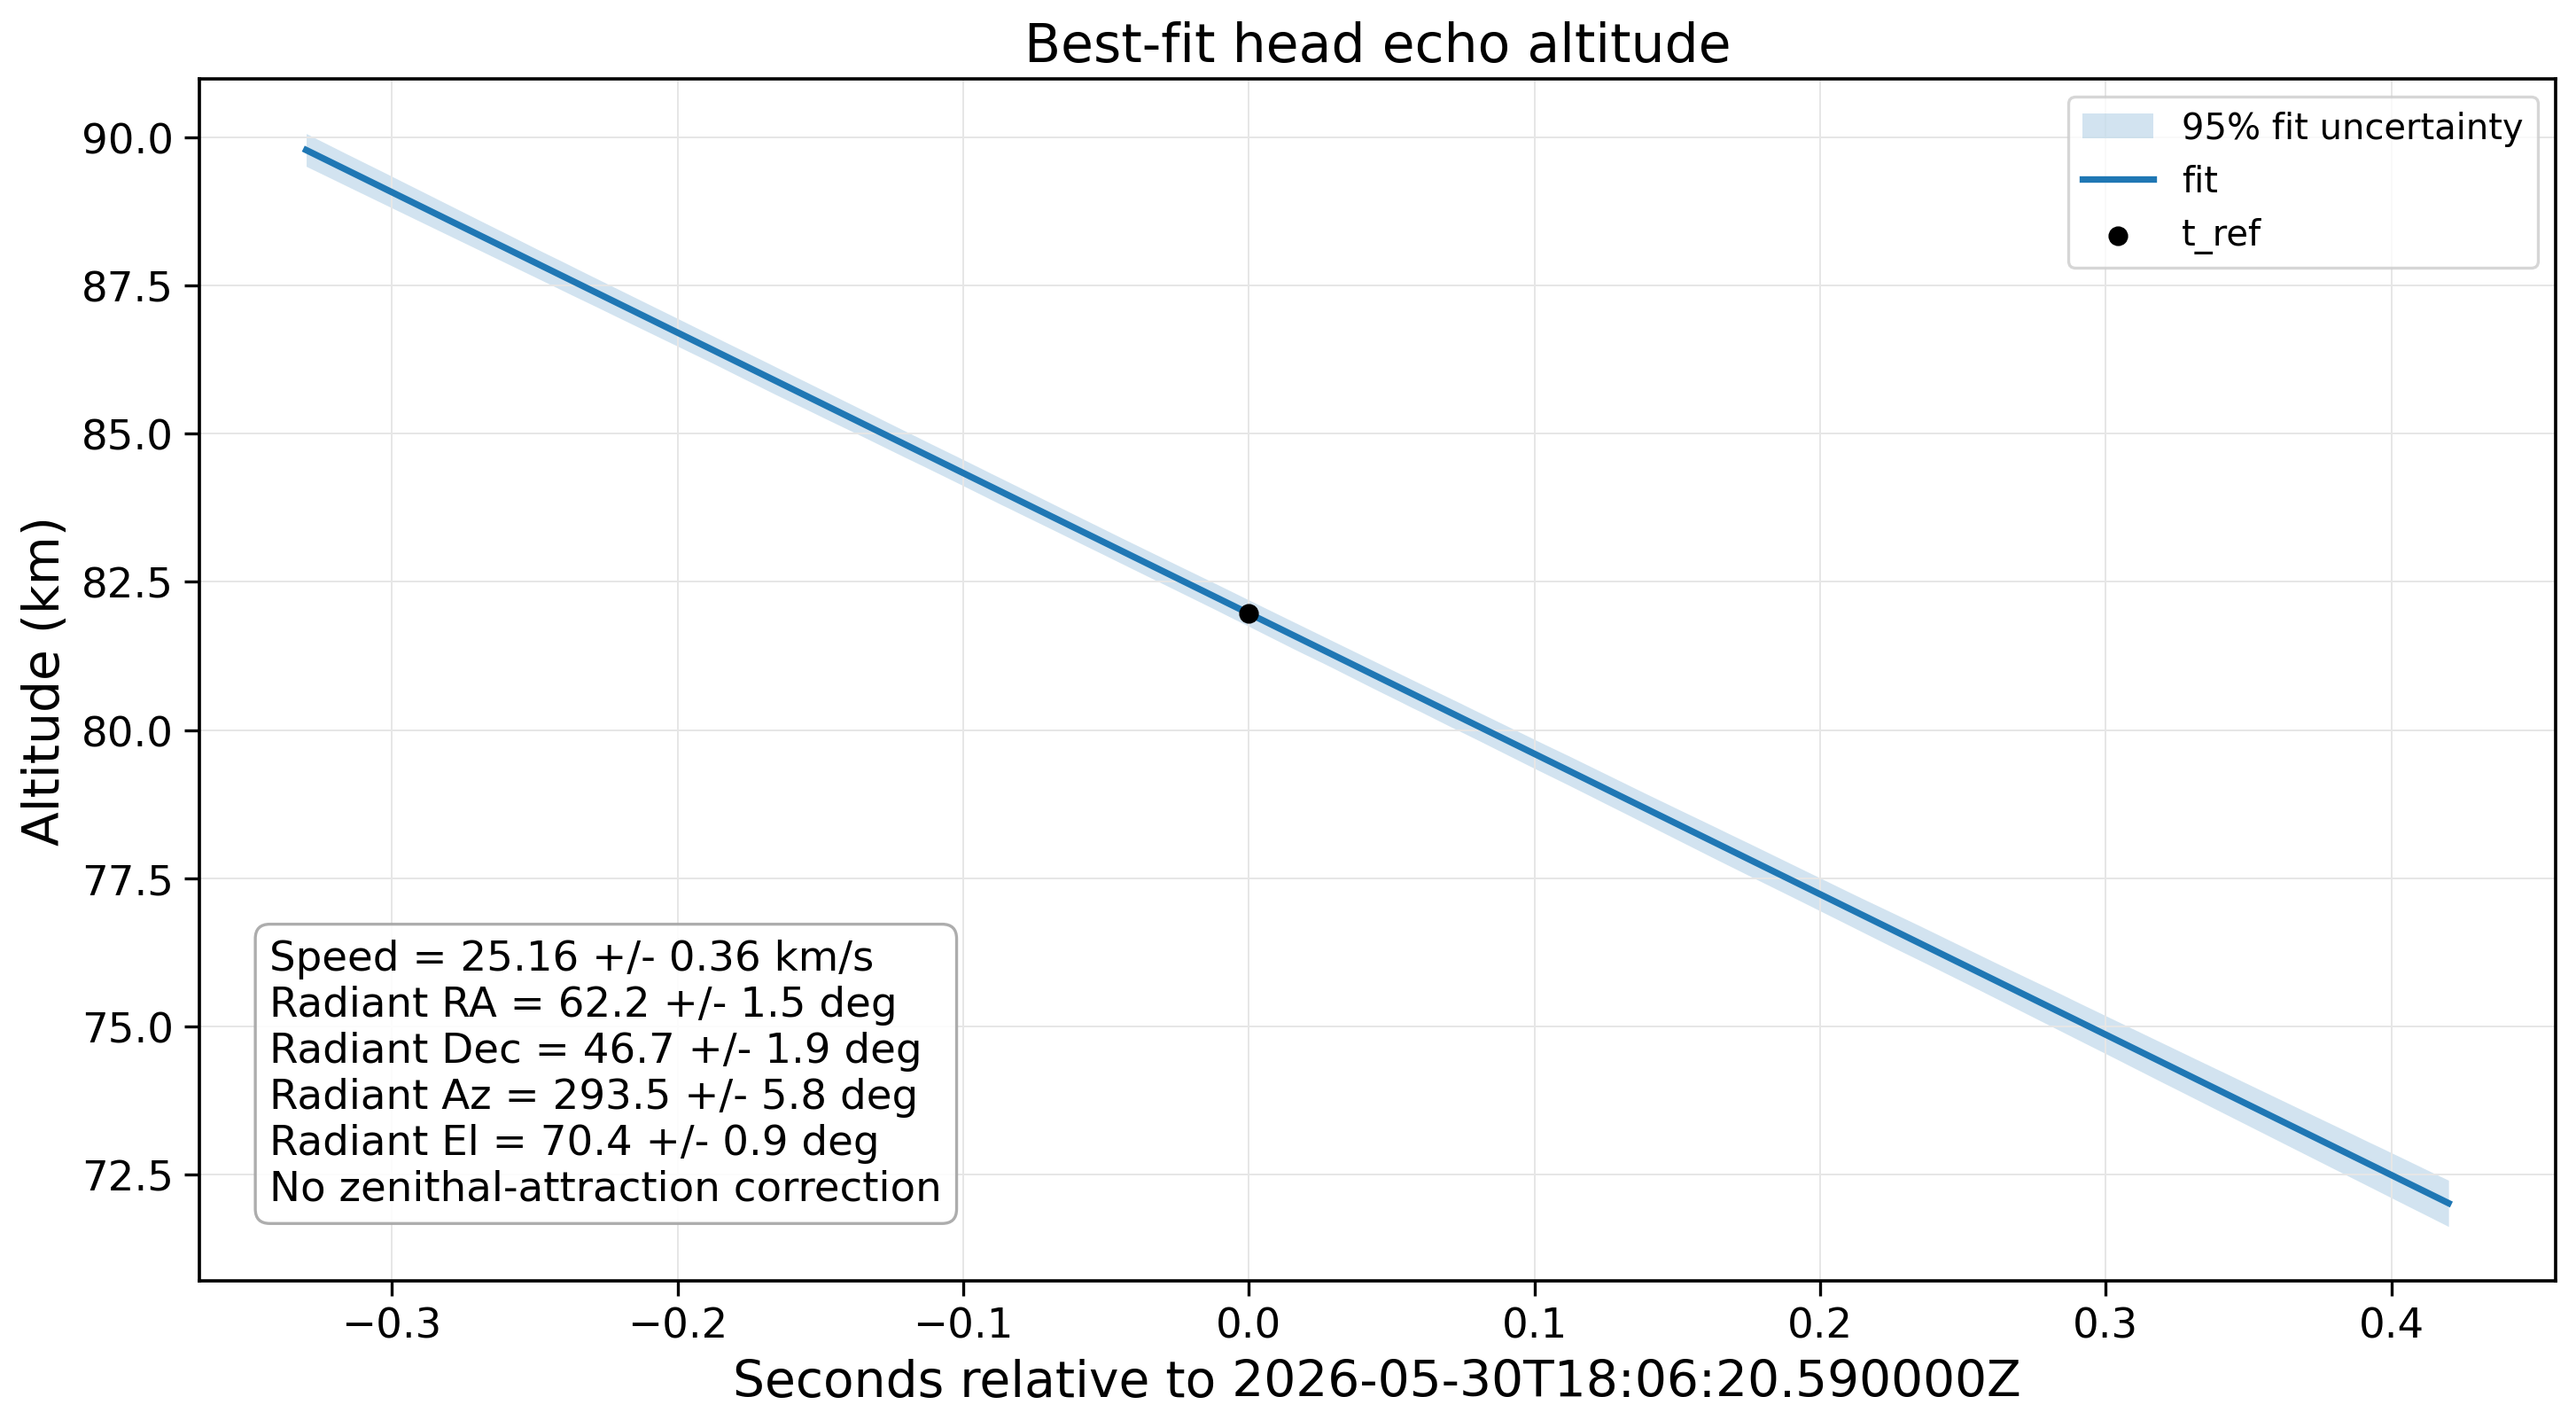
\includegraphics[width=\linewidth]{figures/head_echo_altitude_velocity.png}
  \caption{Altitude implied by the straight-line fit over the retained
  head-echo detection interval.  The text inset gives the fitted absolute
  speed and apparent radiant in RA/Dec and Az/El, including 1-sigma
  uncertainty from covariance samples.  No zenithal-attraction correction has
  been applied.  Shaded bands show sampled 95\% fit uncertainty from the
  linearized least-squares covariance.}
  \figsource{reports/generate_trajectory_report_assets.py}
  \label{fig:trajectory-altitude}
\end{figure}

A second trajectory solution was computed in an inertial frame by combining
the timed head-echo range/Doppler measurements with the non-specular trail echo
positions.  The frame transformation uses a fast Greenwich mean sidereal time
rotation between ECEF and ECI coordinates; the full Astropy GCRS/ITRS
transformation is unnecessary over this several-second arc and is too slow for
iterating on the fit diagnostics.  Most trail echoes are treated as
point-on-path constraints only: the plasma position constrains the spatial
line followed by the meteoroid, but not the time at which the meteoroid passed
that point.  Below 60 km altitude, however, the non-specular trail echoes are
relatively prompt and decay quickly.  For those low-altitude trail points, the
fit also constrains the echo occurrence time to lag the meteoroid passage time
by \(1\pm1\) s.

The straight-line ECI state is
\({\bf p}=({\bf r}_0,{\bf v})\), and the fitted path is
\({\bf r}(t)={\bf r}_0+{\bf v}(t-t_0)\).  For head-echo measurement \(i\), the
model predicts bistatic range \(\rho_i({\bf p})\) and Doppler
\(f_i({\bf p})\).  For trail position \({\bf y}_j\), the closest-path time is
\[
  \tau_j =
  \frac{{\bf v}\cdot({\bf y}_j-{\bf r}_0)}{{\bf v}\cdot{\bf v}},
\]
and the point-to-path residual vector is
\[
  {\bf d}_j({\bf p}) =
  {\bf r}_0 + {\bf v}\tau_j - {\bf y}_j .
\]
The least-squares objective minimized after outlier rejection is
\[
  \begin{aligned}
  \chi^2({\bf p}) ={}&
    \sum_i \left[
      \frac{\rho_i({\bf p})-\rho_i^{\mathrm{obs}}}{\sigma_\rho}
    \right]^2
    +
    \sum_i \left[
      \frac{f_i({\bf p})-f_i^{\mathrm{obs}}}{\sigma_f}
    \right]^2 \\
  &+
    \sum_j
    \frac{\|{\bf d}_j({\bf p})\|^2}{\sigma_{\mathrm{trail}}^2}
    +
    \sum_{j:\,h_j<60\,\mathrm{km}}
    \left[
      \frac{t_j^{\mathrm{echo}}-(t_0+\tau_j+1\,\mathrm{s})}{1\,\mathrm{s}}
    \right]^2 .
  \end{aligned}
\]
The numerical solve uses a soft-\(\ell_1\) loss, but the covariance and plotted
uncertainty samples use the final linearized least-squares Jacobian.  The
measurement scales are estimated from the fit residuals and then applied in a
final fit iteration: \(\sigma_\rho=573\) m, \(\sigma_f=81\) Hz, and
\(\sigma_{\mathrm{trail}}=1.09\) km per trail-position component.  The
low-altitude timing term contributes 21 residuals.

The combined fit admits trail positions between 20 and 115 km altitude.  It
used 181 head-echo measurements and 139 trail positions; four trail positions
were rejected as line-distance outliers.  The resulting residual RMS values are
547 m in head-echo range and 80 Hz in head-echo Doppler, while the retained
trail positions have a median perpendicular distance of 1.49 km and a 95th
percentile distance of 3.88 km.

A physically motivated ballistic propagation fit was then computed by replacing
the straight-line motion model with central Earth gravity and atmospheric drag.
The fitted state is \({\bf y}=({\bf r},{\bf v})\), propagated according to
\[
  \begin{aligned}
    \dot{\bf r} &= {\bf v},\\
    \dot{\bf v} &=
      -\frac{\mu_E}{\|{\bf r}\|^3}{\bf r}
      -\frac{1}{2}\rho(h)\frac{C_D A}{m}
      \|{\bf v}-{\bf v}_{\mathrm{atm}}\|
      ({\bf v}-{\bf v}_{\mathrm{atm}}),
  \end{aligned}
\]
where \({\bf v}_{\mathrm{atm}}={\boldsymbol\omega}_E\times{\bf r}\) assumes a
co-rotating atmosphere.  The atmospheric density \(\rho(h)\) is taken from an
MSIS altitude profile when available, with an exponential fallback.  The
optimized drag parameter is a single constant \(C_D A/m\), initialized from the
combined straight-line solution and fit together with the reference position
and velocity.  The fitted value is
\(C_D A/m = 8.45\times10^{-4}\ \mathrm{m^2\,kg^{-1}}\).  The retained trail
positions have a median distance of 1.81 km from the ballistic trajectory.

For the fall-line extrapolation, the fitted ballistic trajectory is propagated
to 30 km altitude.  The radar trail measurements near this altitude constrain
the position and direction of the path immediately before dark flight, but the
subsequent sea-level impact depends on the size distribution of surviving
fragments.  A nominal 10 cm diameter spherical fragment of density
\(3000\ \mathrm{kg\,m^{-3}}\) is used as a reference case.  With \(C_D=1\), this
gives
\[
  \frac{C_D A}{m}
  =
  \frac{3C_D}{2d\rho_m}
  =
  0.005\ \mathrm{m^2\,kg^{-1}} .
\]
In this nominal extrapolation, the trajectory reaches 30 km altitude at
18:06:22.75 UTC and the 10 cm fragment reaches sea level at 18:11:16.93 UTC
with a speed of about 351 m s\(^{-1}\).  To represent the unknown surviving
fragment size, Figure~\ref{fig:ballistic-impact-map} and
Table~\ref{tab:fragment-impact} also sample fragment diameters from 1 to
100 cm at fixed density, combined with samples from the linearized covariance
of the ballistic fit.  The resulting spread should be interpreted as a large
dark-flight uncertainty, not as a precise strewn-field prediction.

\begin{figure}
  \centering
  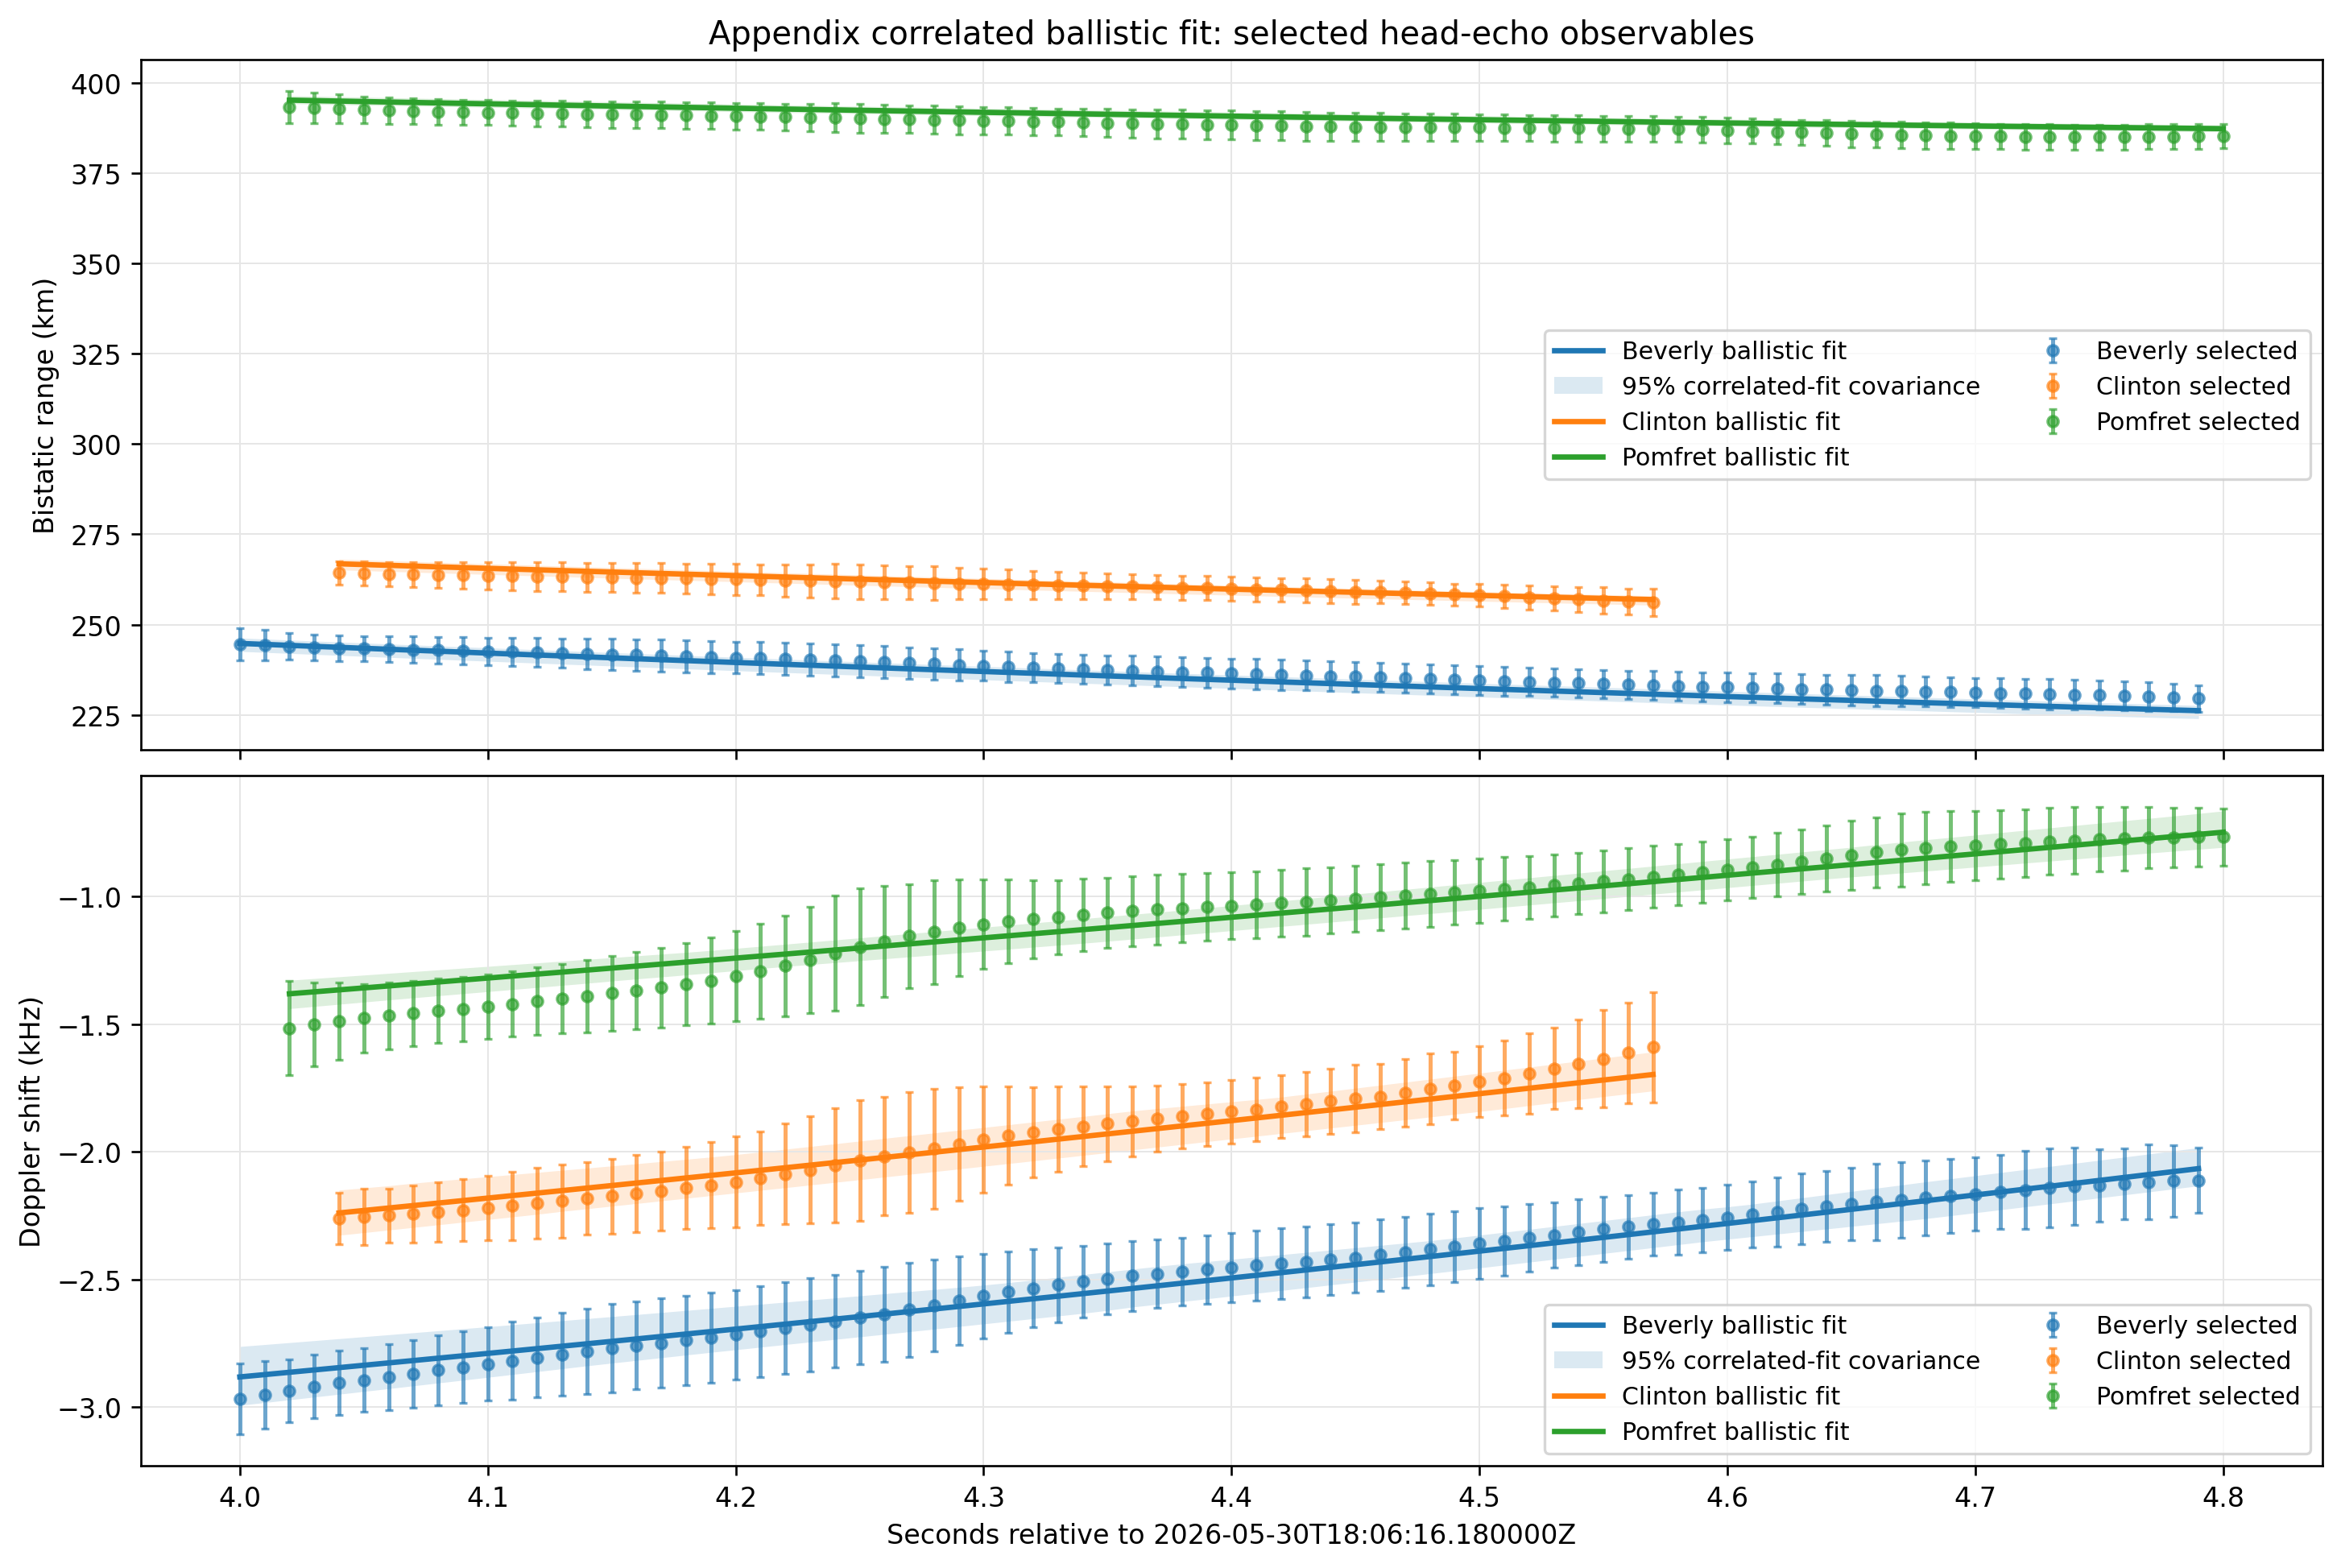
\includegraphics[width=\linewidth]{figures/combined_head_trail_range_doppler_fit.png}
  \caption{Range and Doppler measurements for the combined ECI head/trail
  trajectory fit.  Points show the timed head-echo measurements; lines show
  the fitted bistatic range and Doppler model.  Shaded bands show sampled
  95\% uncertainty from the combined-fit covariance.}
  \figsource{fit_combined_head_trail_eci.py}
  \label{fig:combined-trajectory-observables}
\end{figure}

\begin{figure}
  \centering
  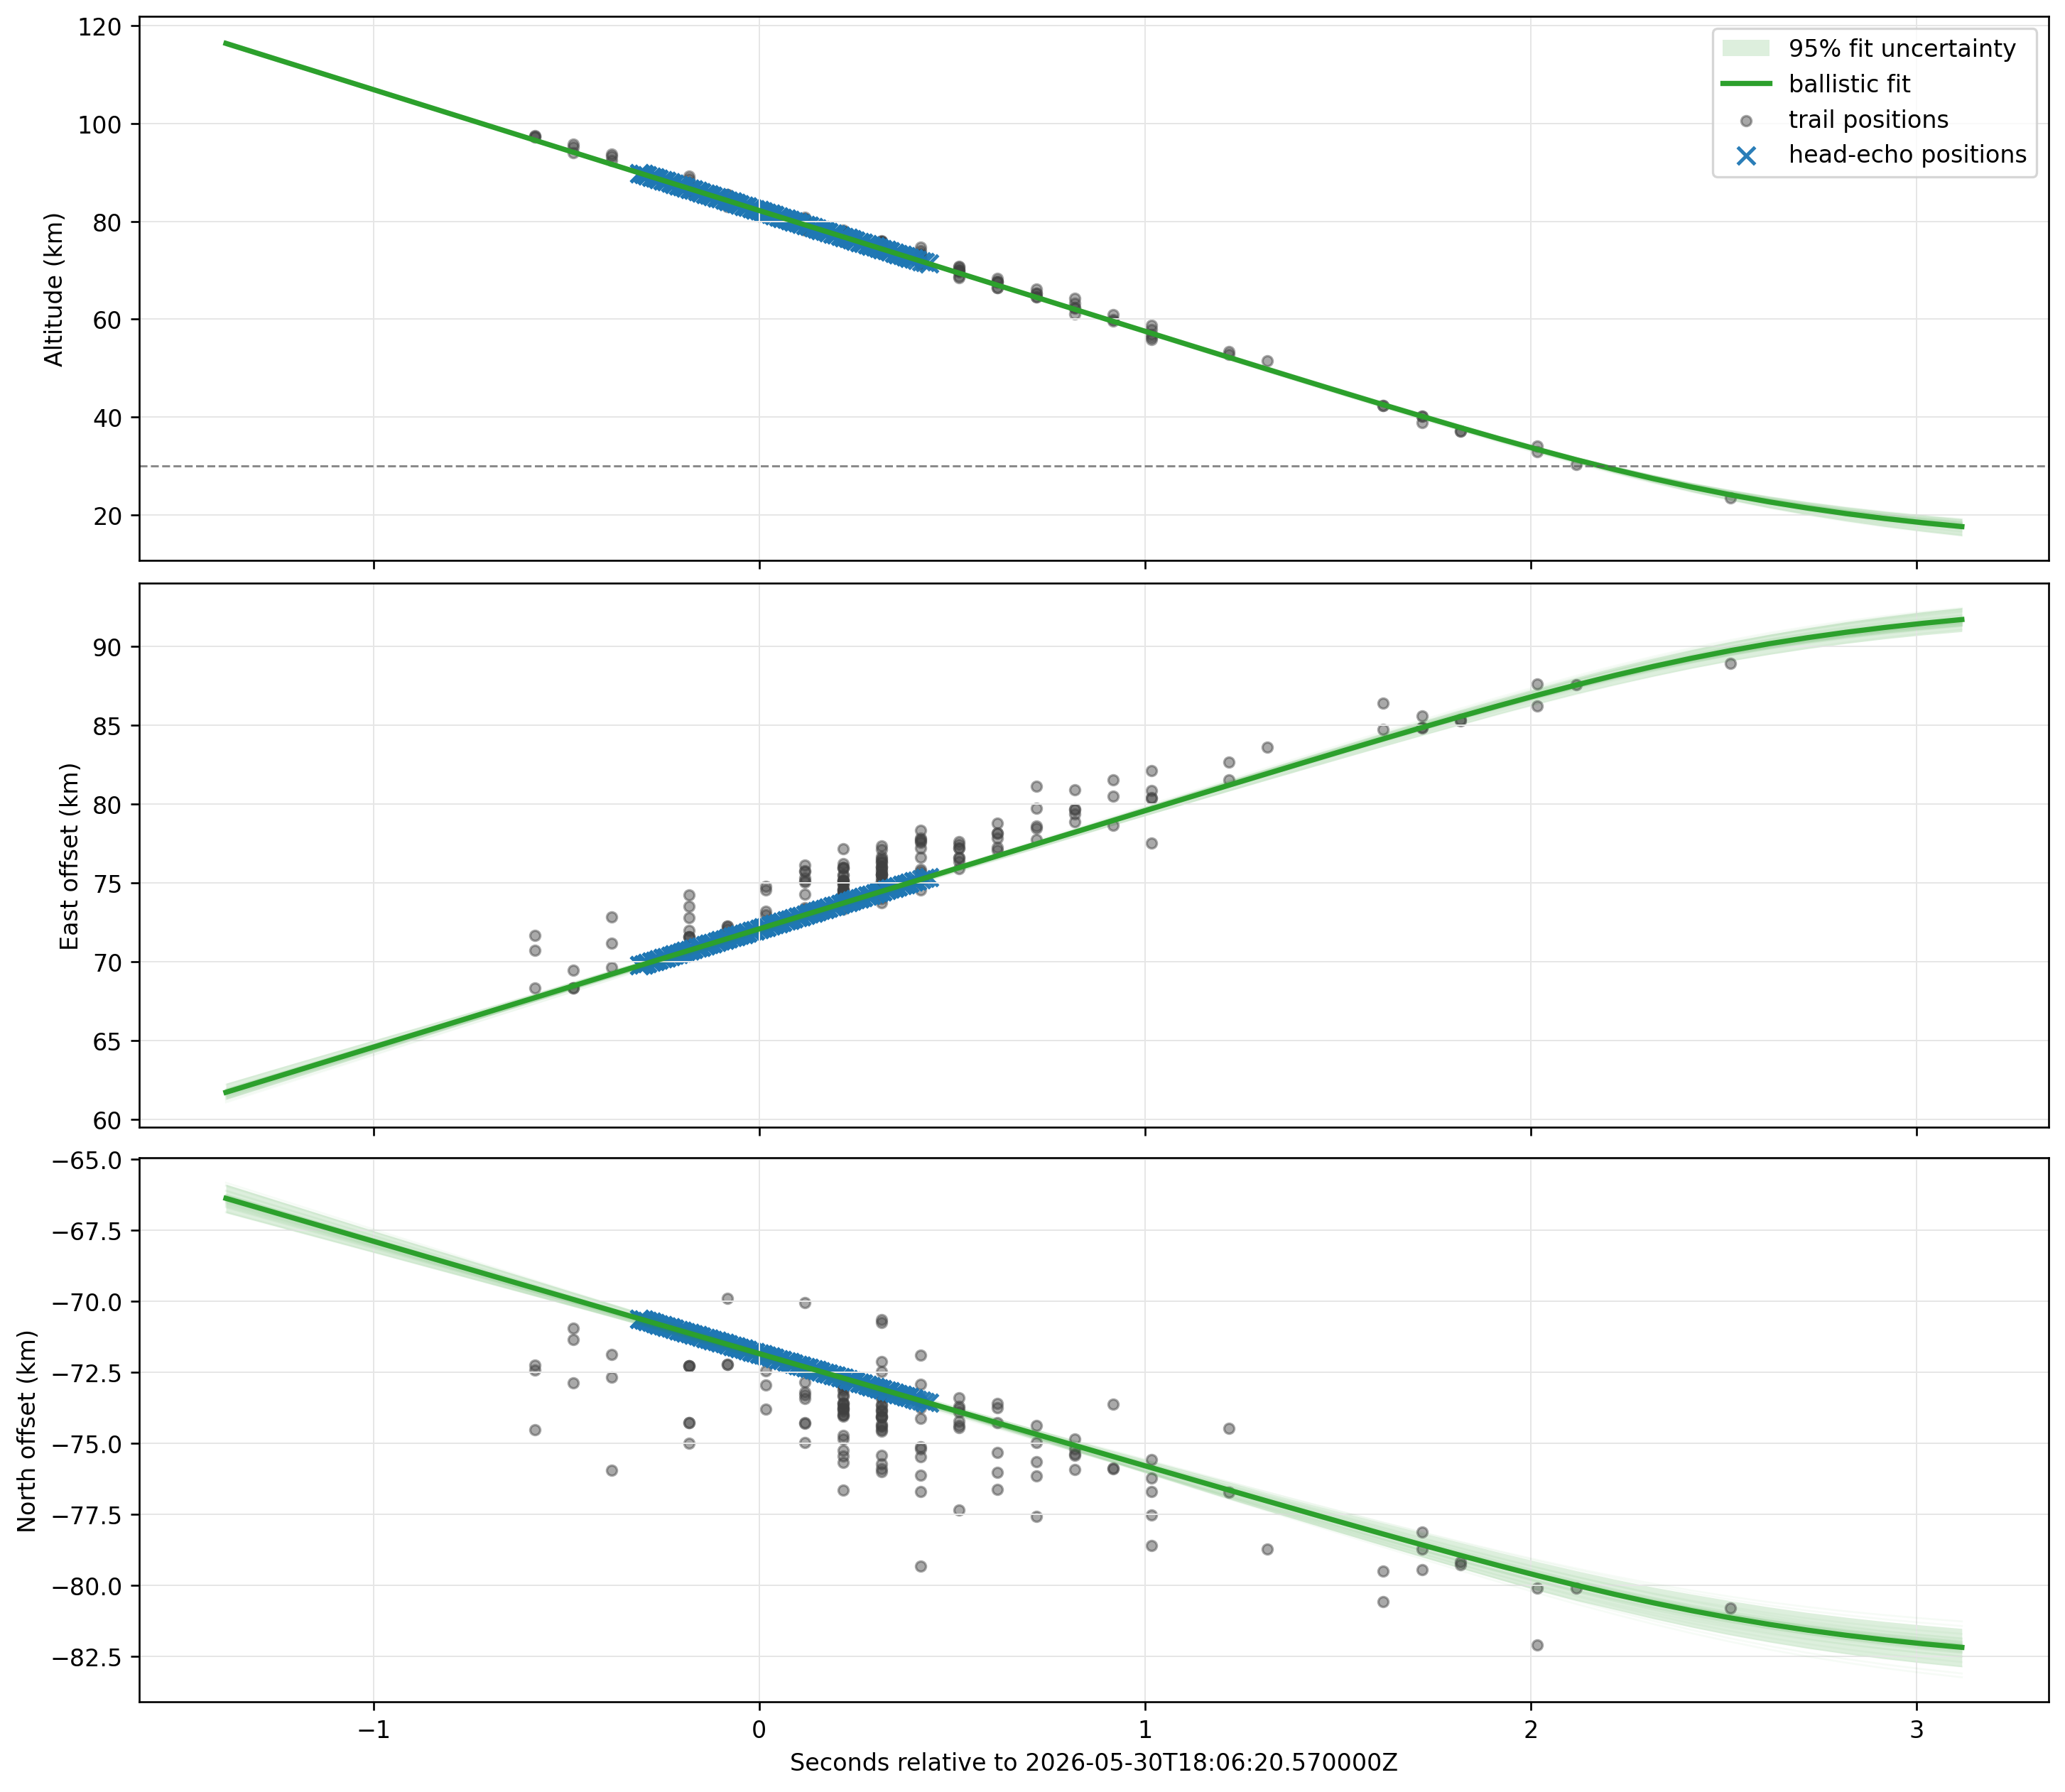
\includegraphics[width=\linewidth]{figures/ballistic_head_trail_altitude_enu.png}
  \caption{Ballistic trajectory in the transmitter ENU frame.  The green curve
  shows the best-fit ballistic trajectory through the head-echo and retained
  trail region; the shaded band and faint green curves show samples from the
  linearized fit covariance.  Blue crosses show head-echo-derived positions and
  gray points show non-specular trail positions projected to the closest point
  on the trajectory.  The dashed line marks 30 km altitude, where the nominal
  fragment model used for the impact estimate in Figure~\ref{fig:ballistic-impact-map}
  begins.}
  \figsource{fit_ballistic_head_trail.py}
  \label{fig:ballistic-trajectory-altitude}
\end{figure}

\begin{figure}
  \centering
  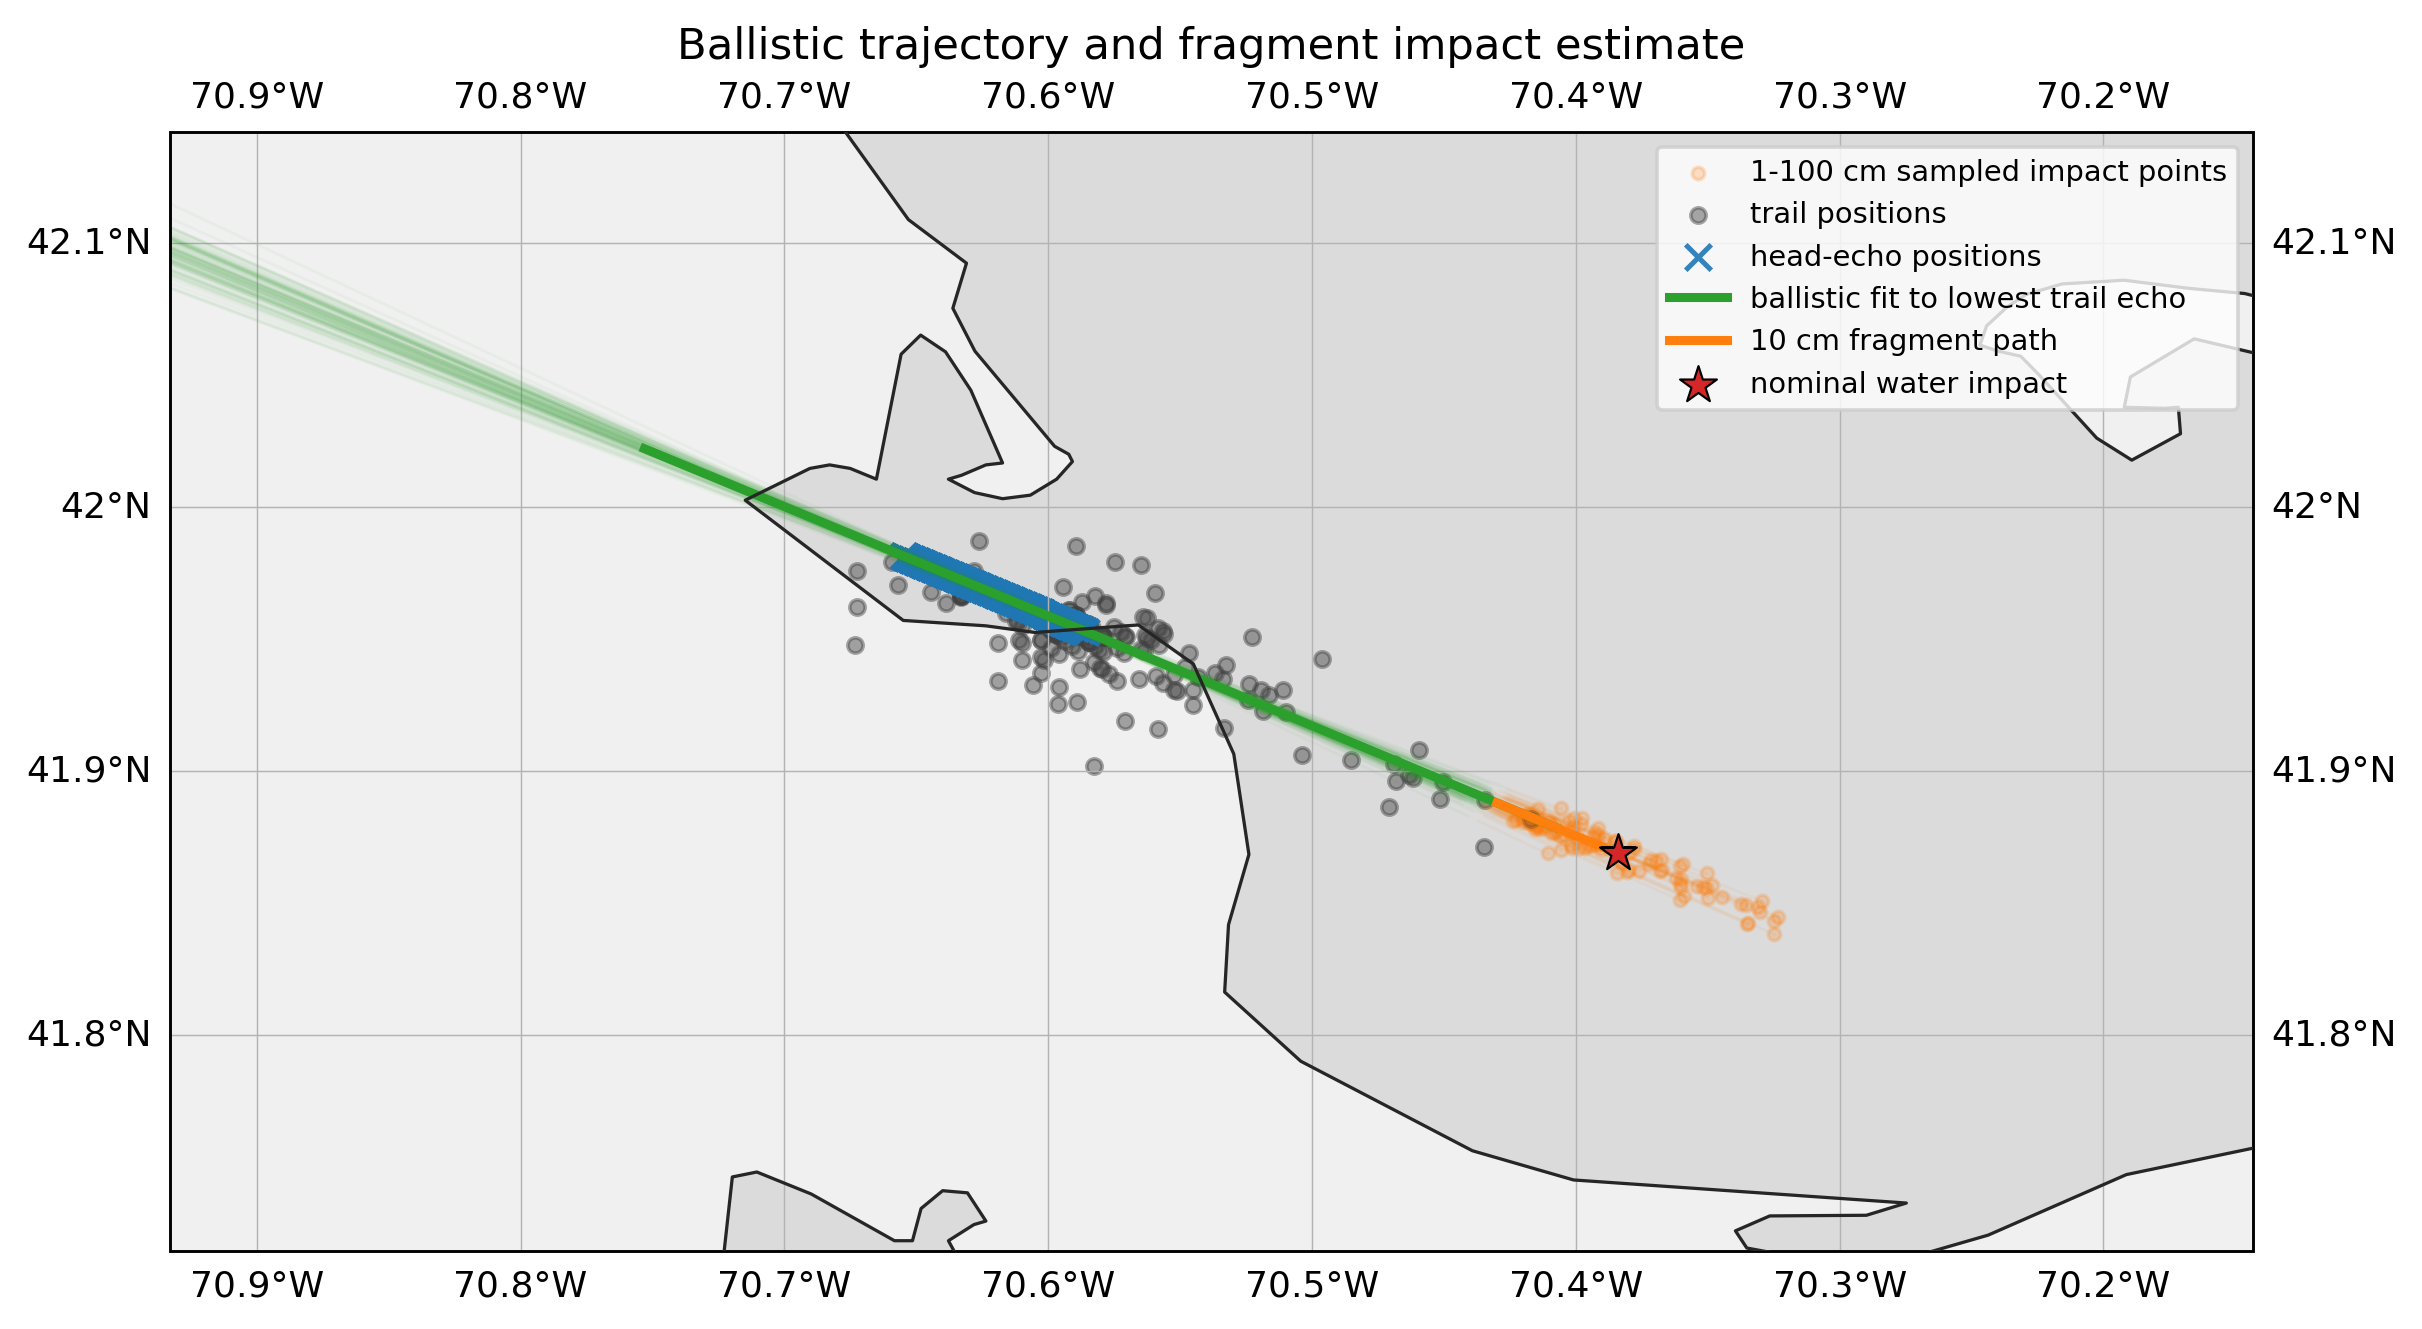
\includegraphics[width=\linewidth]{figures/ballistic_head_trail_impact_map.png}
  \caption{Ballistic trajectory and fragment-impact estimate.  The
  green curve shows the best-fit ballistic trajectory extended to the altitude
  of the lowest retained non-specular trail echo.  The orange curve is only the
  ground-fall extrapolation: below 30 km the object is assumed to have broken
  into 10 cm diameter spherical fragments of density
  \(3000\ \mathrm{kg\,m^{-3}}\), propagated with \(C_D=1\) so that
  \(C_D A/m = 0.005\ \mathrm{m^2\,kg^{-1}}\).  Orange points show sea-level
  impact samples obtained by varying the fragment diameter from 1 to 100 cm
  and sampling the ballistic-fit covariance.  The red star marks the nominal
  10 cm water-impact point in Cape Cod Bay.}
  \figsource{fit_ballistic_head_trail.py}
  \label{fig:ballistic-impact-map}
\end{figure}

\begin{table}[ht]
  \centering
  \caption{Sea-level impact estimate for the nominal 10 cm fragment and for fragment diameters sampled between 1 and 100 cm.  The sampled interval includes the linearized ballistic fit covariance and the unknown post-30 km fragment size at fixed density \(3000\ \mathrm{kg\,m^{-3}}\).}
  \label{tab:fragment-impact}
  \resizebox{\linewidth}{!}{%
  \begin{tabular}{lll}
    \toprule
    Quantity & Nominal 10 cm fragment & 95\% sampled interval \\
    \midrule
    Latitude (deg) & 41.8718 & 41.8747 [41.8480, 41.8878] \\
    Longitude (deg) & -70.3796 & -70.3895 [-70.4128, -70.3238] \\
    Sea-level time (UTC) & 18:11:18.9564 & 18:12:33.5408 [18:07:00.4247, 18:23:37.2135] \\
    Fall time below 30 km (s) & 296 & 371 [38, 1034] \\
    Impact speed (m s$^{-1}$) & 351 & 350 [347, 397] \\
    Fragment diameter (cm) & 10.0 & 7.0 [1.1, 85.3] \\
    \bottomrule
  \end{tabular}
  }
\end{table}


\begin{figure}
  \centering
  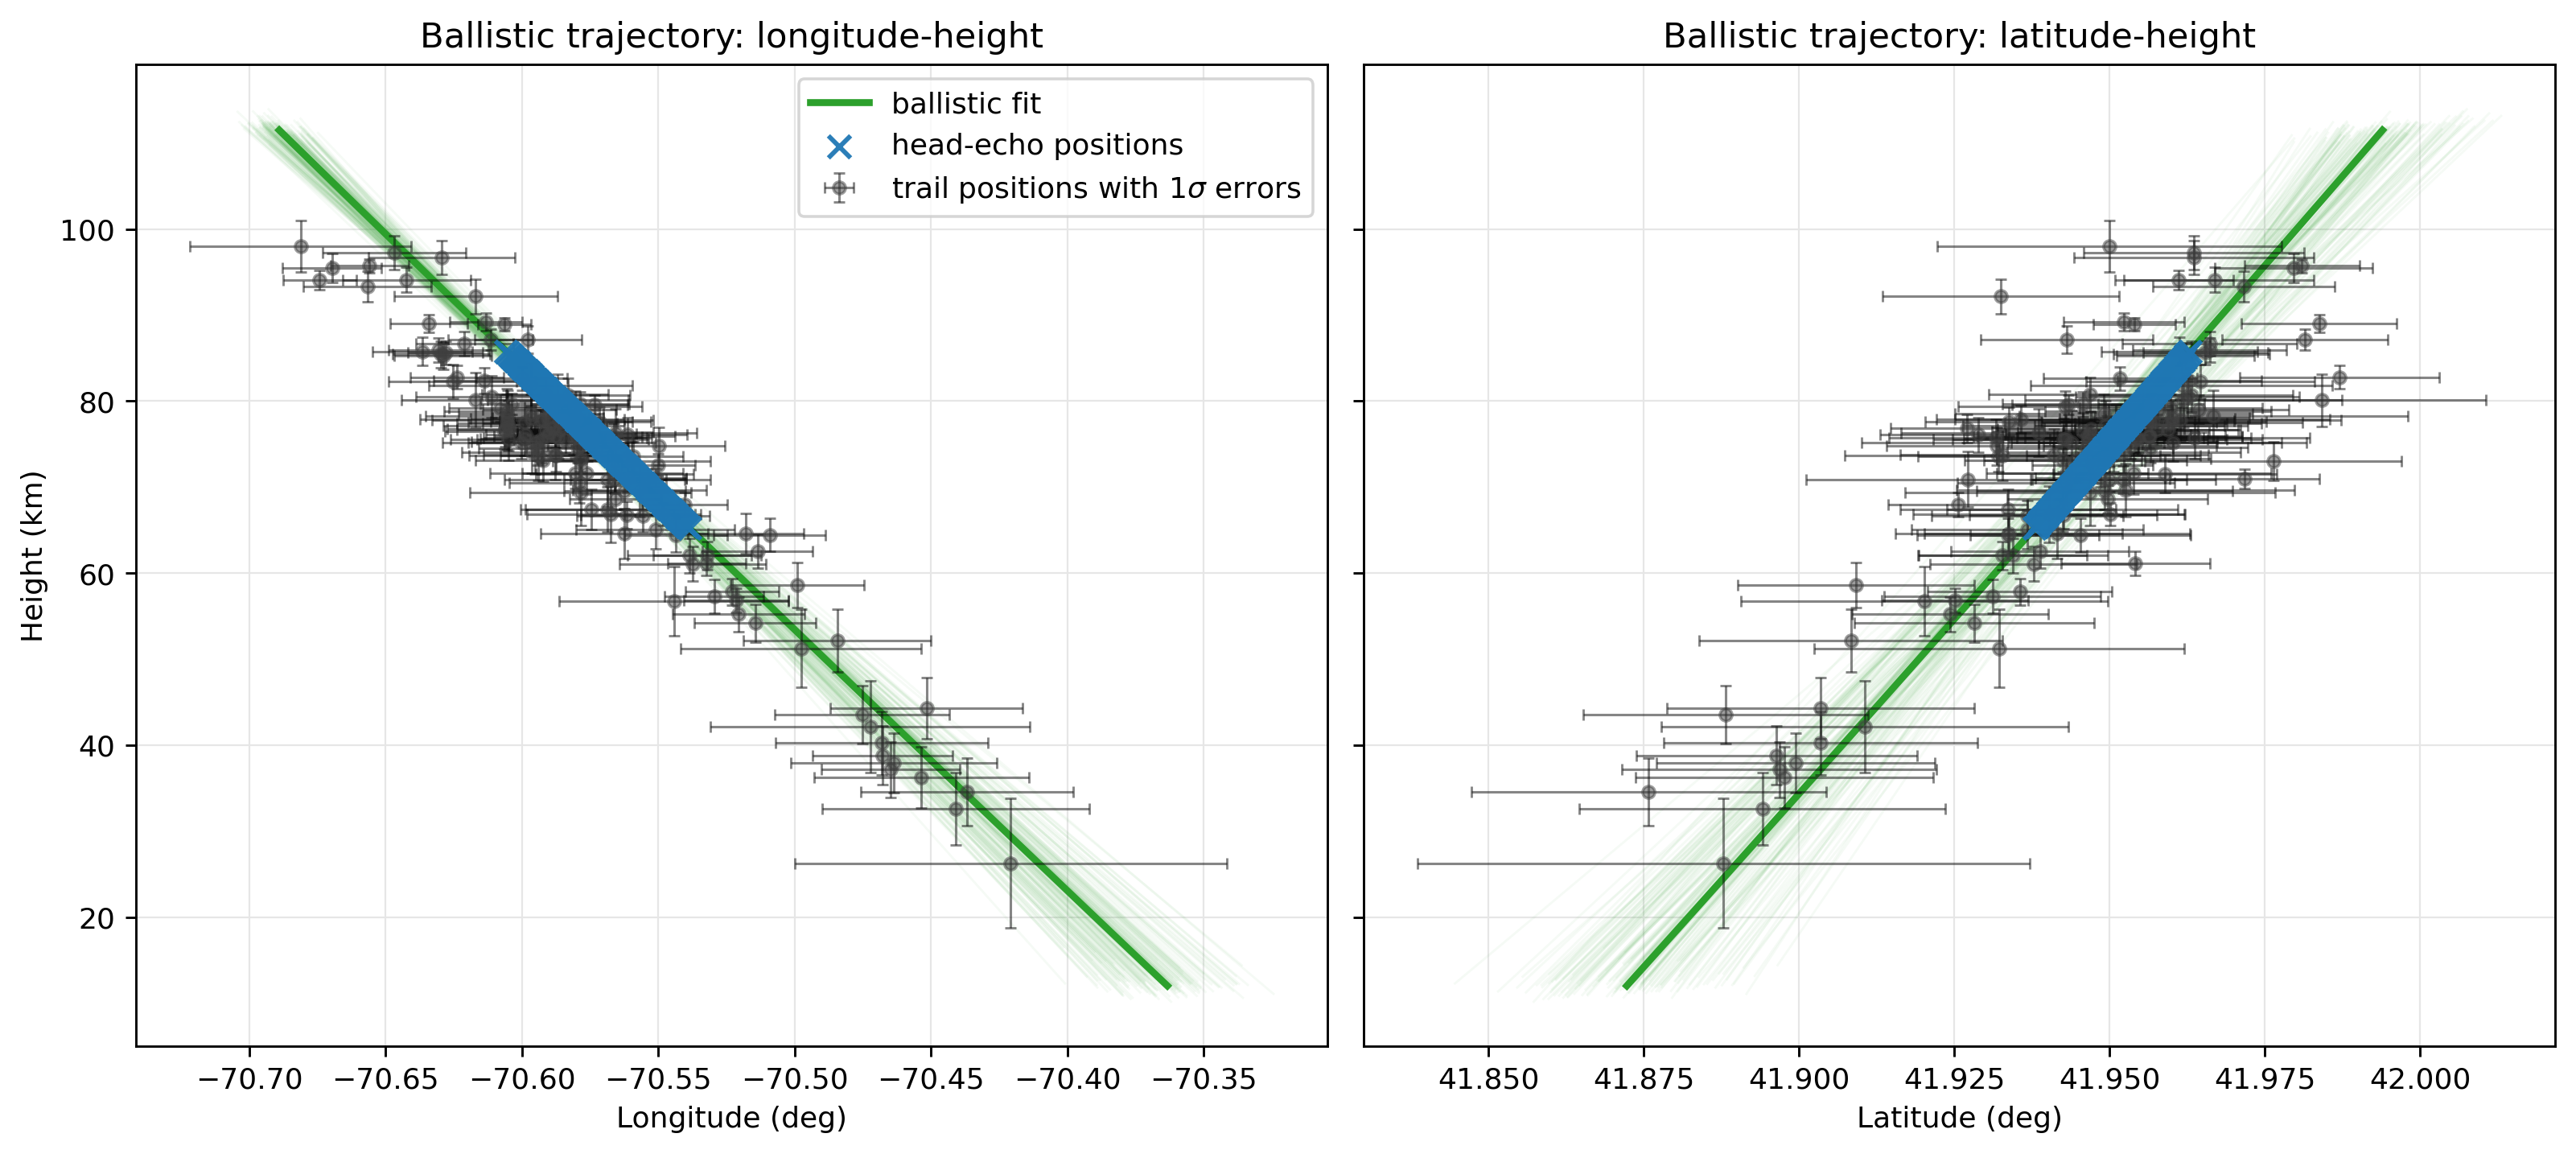
\includegraphics[width=\linewidth]{figures/ballistic_head_trail_lonlat_height.png}
  \caption{Ballistic head/trail trajectory fit shown as longitude versus height
  and latitude versus height.  The green curve is the best-fit trajectory under
  central gravity and fitted atmospheric drag; faint green curves are samples
  from the linearized fit covariance.  Gray points show retained non-specular
  trail positions, and blue crosses show head-echo-derived positions along the
  ballistic solution.}
  \figsource{fit_ballistic_head_trail.py}
  \label{fig:ballistic-lonlat-height}
\end{figure}

\begin{figure}
  \centering
  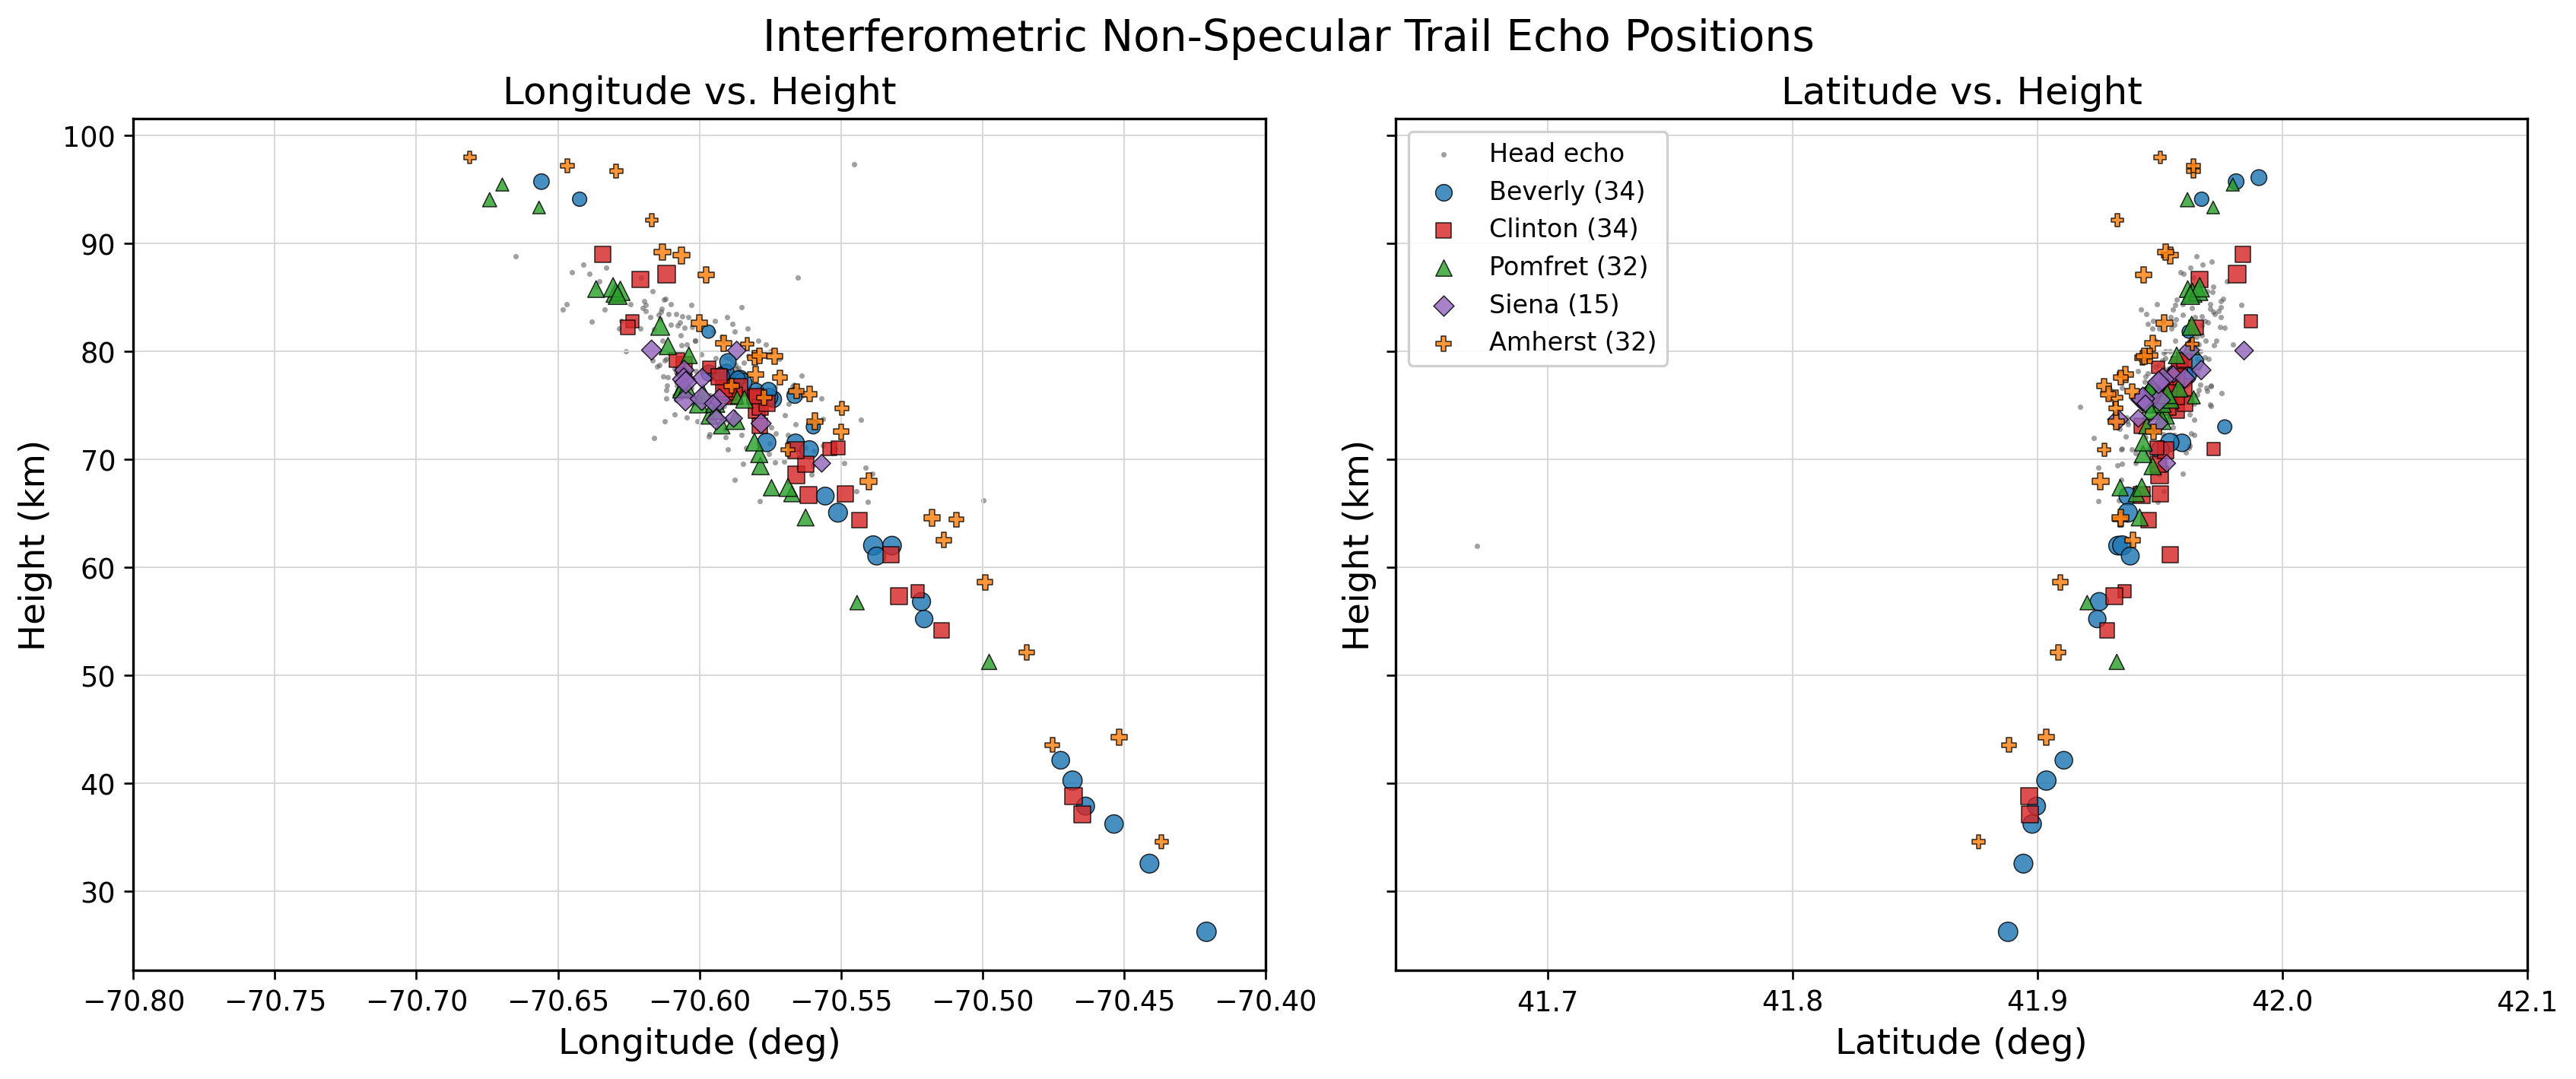
\includegraphics[width=\linewidth]{figures/trail_echo_geographic_height.png}
  \caption{Interferometric non-specular trail echo AoD plus bistatic-delay
  position solutions as a function of longitude and latitude versus height.
  Colors and marker shapes identify the receiving station used for the
  bistatic echo measurement; gray points show the corresponding head-echo AoD
  plus bistatic-delay positions.}
  \figsource{plot_interferometric_echo_geometry.py}
  \label{fig:trail-geographic-height}
\end{figure}

\begin{figure}
  \centering
  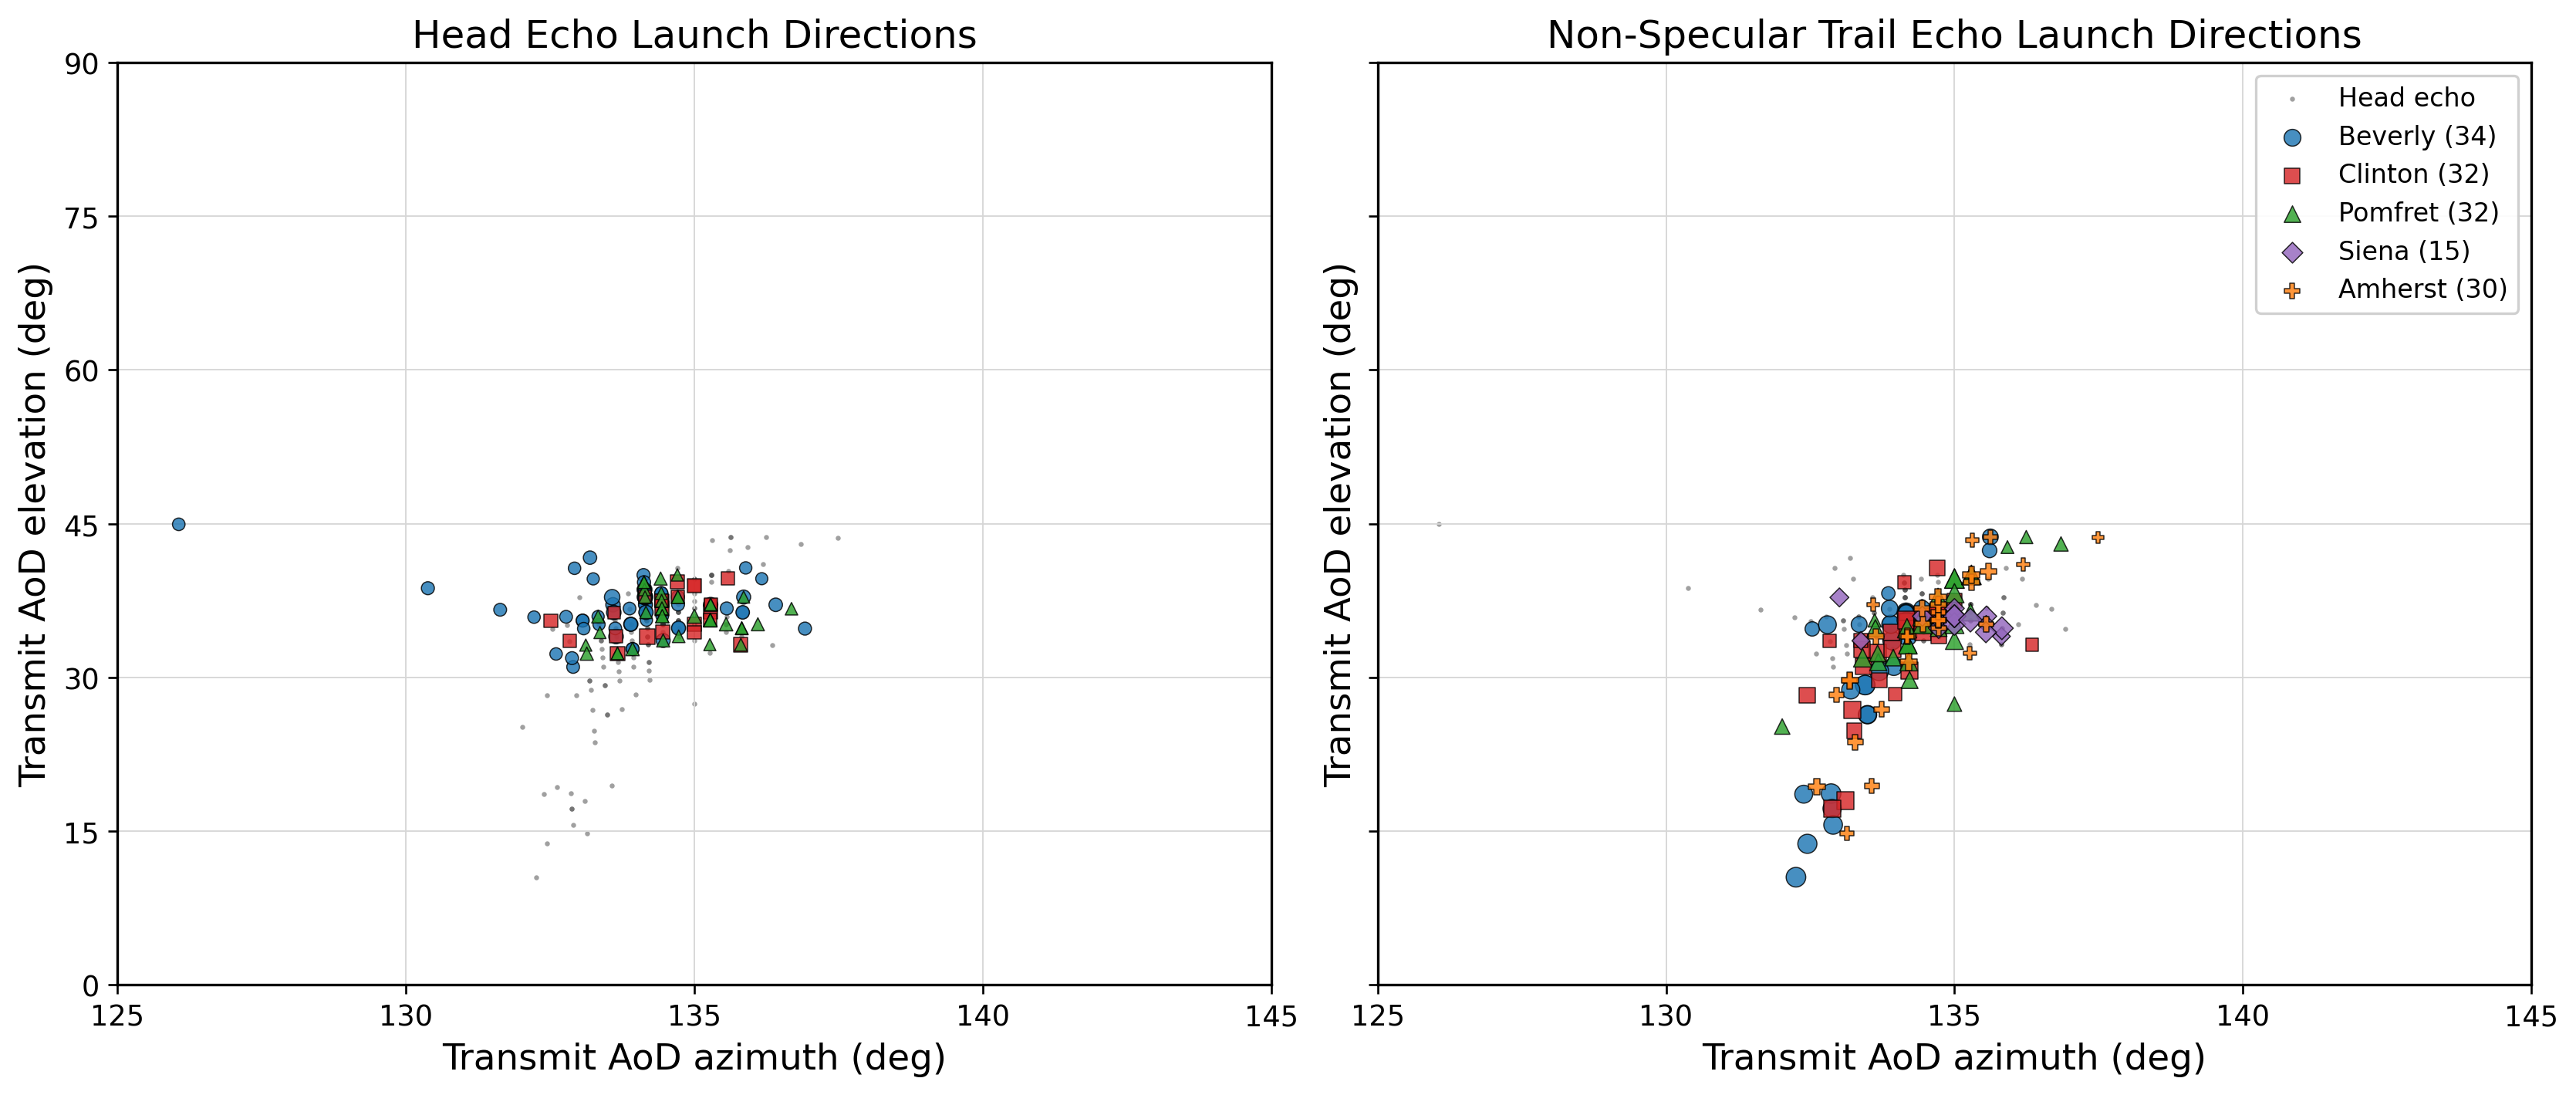
\includegraphics[width=\linewidth]{figures/head_trail_aod_launch_angles.png}
  \caption{Transmit angle-of-departure launch directions inferred by the
  five-antenna interferometer.  The left panel shows head-echo AoD solutions
  matched to the tri-static trajectory fit, and the right panel shows
  near-zero-Doppler non-specular trail echo AoD solutions.  Colors identify
  the receiving station.}
  \figsource{plot_interferometric_echo_geometry.py}
  \label{fig:head-trail-aod-launch}
\end{figure}

\subsection{Orbit and Source Association}

The heliocentric orbit was obtained from the ballistic head/trail fit shown in
Figure~\ref{fig:ballistic-trajectory-altitude}.  The fitted GCRS state at the
ballistic reference epoch was transformed to ITRS/ECEF, propagated backward
with the JPL ephemeris until the object was outside 0.01 AU from Earth, then
converted to Keplerian elements in the heliocentric mean ecliptic frame.  This
orbit was compared with the
local MPC near-Earth asteroid catalogue in \texttt{data/NEA.txt}, the MPC
comet-element catalogue in \texttt{data/cometels.json.gz}, and the 2026 IAU Meteor
Data Center established shower list in
\texttt{data/streamestablisheddata2026.txt}.  The shower comparison uses only
established-shower entries whose reference field contains Jenniskens or Brown.
For comets and showers, the catalogue orbital elements are compared without
using a mean anomaly, because a comet/stream source comparison is based on
orbital-shape similarity rather than a single object at a specified orbital
phase.  The table therefore lists \(a,q,e,i,\omega,\Omega\), the catalogue
geocentric J2000 radiant RA/Dec where available, the Jopek \(D_H\) orbital
dissimilarity, and the angular radiant separation \(\Delta_R\).
The aphelion distance \(Q=a(1+e)\) and the Tisserand parameter with respect to
Jupiter were also computed for meteor-orbit classification.  The latter is
computed from the sampled heliocentric elements as
\[
  T_J = \frac{a_J}{a}
        + 2\cos i \sqrt{\frac{a}{a_J}\left(1-e^2\right)},
\]
where \(a_J=5.20336301~\mathrm{AU}\).  This is the standard circular
restricted three-body form \cite{murray_dermott_1999}.  The
Jopek--Williams sporadic-meteoroid classification was then evaluated using
both the recommended \(Q-i\) rule, cometary if \(Q>4.6~\mathrm{AU}\) or
\(i>75^\circ\), and the corresponding \(T_J-i\) rule, cometary if
\(T_J<3.0\) or \(i>75^\circ\) when written with the standard Jupiter
Tisserand parameter \cite{jopek_williams_2013}.  These rules are population
classifiers rather than parent-body identifications.  For comparison, the
Canadian Meteor Orbit Radar survey convention of \textcite{brown_2008_cmor}
was also applied: \(T_J>3\) is asteroidal, \(2<T_J<3\) is Jupiter-family
comet-like, and \(T_J<2\) is Halley-type or long-period comet-like.
The orbital uncertainties are obtained by drawing 200 states from the
six-parameter state marginal of the ballistic-fit covariance and propagating
each sample independently.  Thus the ballistic fit shown in
Figure~\ref{fig:ballistic-trajectory-altitude} is the source of the
orbit-element, \(v_g\), and corrected-radiant uncertainties in
Table~\ref{tab:orbit-parameters} and Figure~\ref{fig:orbit-xy}.

\begin{figure}
  \centering
  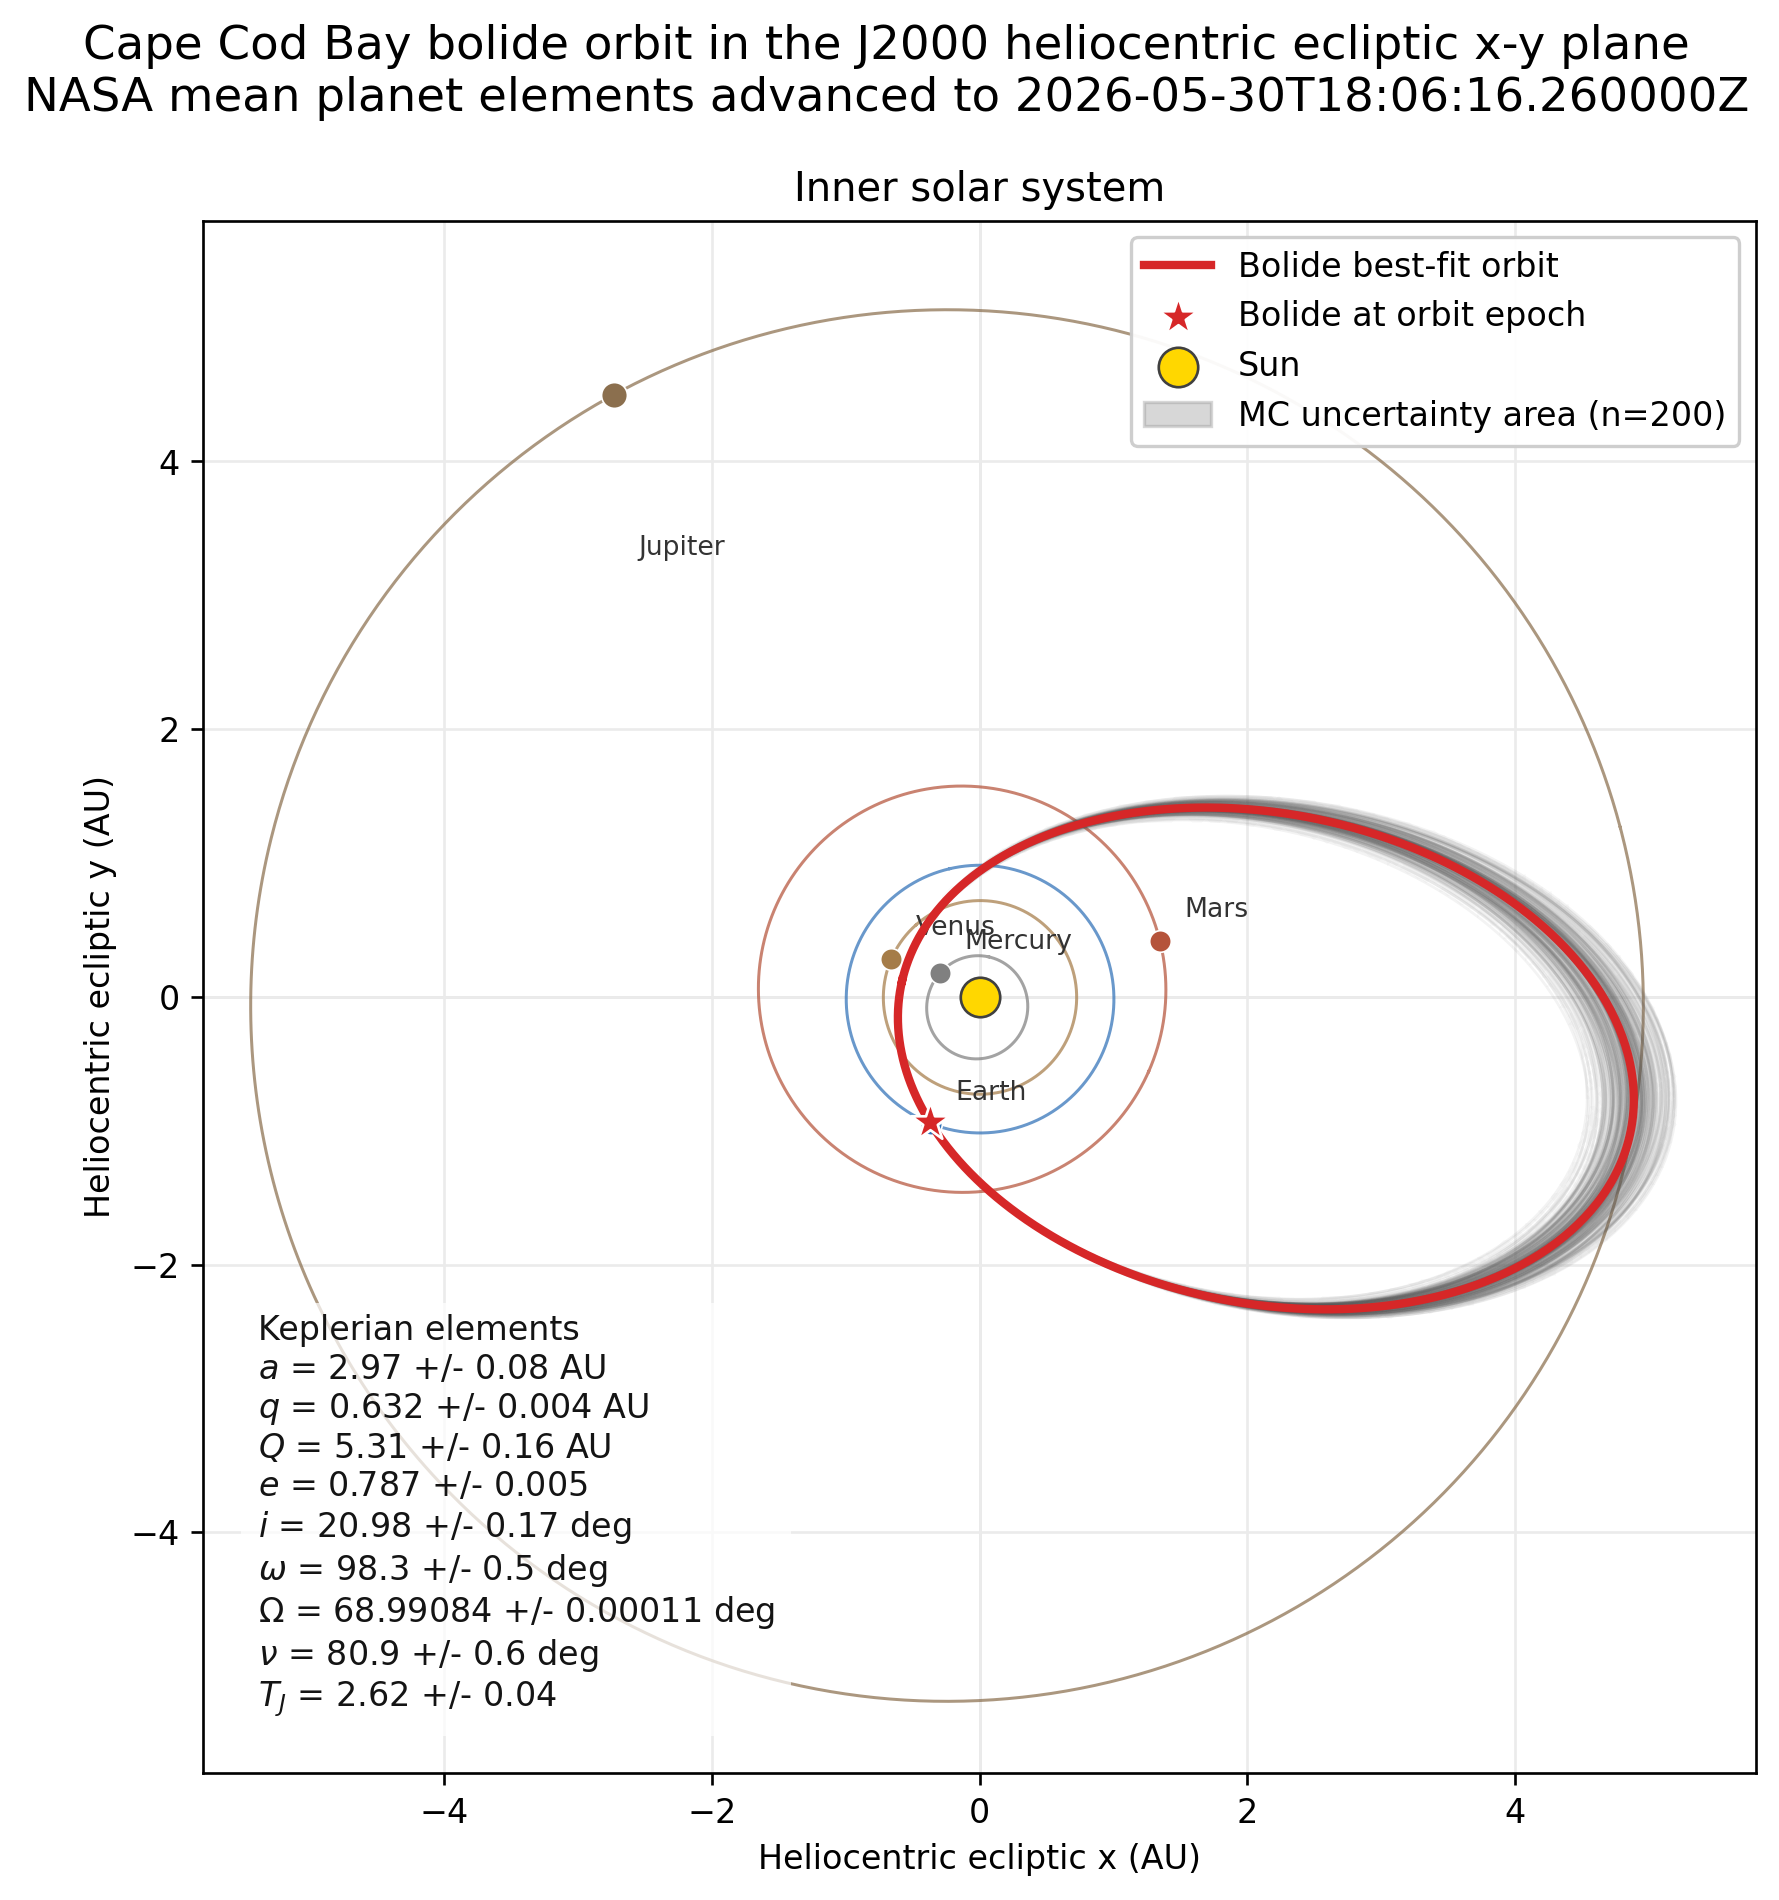
\includegraphics[width=\linewidth]{figures/orbit_xy_bolide.png}
  \caption{Best-fit bolide orbit in the J2000 heliocentric ecliptic \(x\)--\(y\)
  plane.  The plot zooms into the inner solar system and shows the Monte Carlo
  orbit uncertainty envelope from 200 ballistic-fit covariance samples with NASA
  mean planet elements advanced to the bolide epoch.}
  \figsource{plot_orbit_xy.py}
  \label{fig:orbit-xy}
\end{figure}

\begin{table}
  \centering
  \caption{Bolide heliocentric mean-ecliptic orbital elements and corrected
  geocentric speed, radiant, and Tisserand parameter with respect to Jupiter
  with 1-sigma Monte Carlo uncertainties propagated from the ballistic-fit
  state covariance.}
  \resizebox{0.78\linewidth}{!}{\begin{tabular}{llrl}
\toprule
Quantity & Symbol & Unit & Estimate \\
\midrule
Semimajor axis & $a$ & AU & 2.89 $\pm$ 0.07 \\
Perihelion distance & $q$ & AU & 0.628 $\pm$ 0.004 \\
Aphelion distance & $Q$ & AU & 5.16 $\pm$ 0.15 \\
Eccentricity & $e$ &  & 0.783 $\pm$ 0.005 \\
Inclination & $i$ & deg & 21.07 $\pm$ 0.17 \\
Argument of perihelion & $\omega$ & deg & 97.7 $\pm$ 0.6 \\
Longitude of ascending node & $\Omega$ & deg & 68.99081 $\pm$ 0.00011 \\
True anomaly at epoch & $\nu$ & deg & 81.6 $\pm$ 0.6 \\
Geocentric speed & $v_g$ & km s$^{-1}$ & 24.61 $\pm$ 0.11 \\
Tisserand parameter with respect to Jupiter & $T_J$ &  & 2.67 $\pm$ 0.04 \\
Corrected radiant right ascension & RA & deg & 59.88 $\pm$ 0.25 \\
Corrected radiant declination & Dec & deg & 48.56 $\pm$ 0.29 \\
Radiant azimuth at 100 km & Az & deg & 299.2 $\pm$ 0.9 \\
Radiant zenith angle at 100 km & $z$ & deg & 19.57 $\pm$ 0.13 \\
Geodetic latitude at 100 km & $\phi_{100}$ & deg & 41.9997 $\pm$ 0.0013 \\
Geodetic longitude at 100 km & $\lambda_{100}$ & deg & -70.6847 $\pm$ 0.0016 \\
Time at 100 km & $t_{100}$ & UTC & 2026-05-30 18:06:19.848 UTC $\pm$ 0.006 s \\
\bottomrule
\end{tabular}
}
  \label{tab:orbit-parameters}
\end{table}

\begin{table}
  \centering
  \caption{Meteor-orbit classification using the Jopek--Williams
  \(Q-i\) and \(T_J-i\) criteria and the Brown et al. \(T_J\)-only population
  divisions.  Fractions are evaluated over the same Monte Carlo orbit samples
  used for Table~\ref{tab:orbit-parameters}.}
  \small
  \renewcommand{\arraystretch}{1.16}
\begin{tabularx}{\linewidth}{@{}>{\raggedright\arraybackslash}p{0.18\linewidth}>{\raggedright\arraybackslash}X>{\raggedright\arraybackslash}p{0.22\linewidth}>{\raggedright\arraybackslash}p{0.20\linewidth}@{}}
\toprule
Criterion & Population rule & Orbit value & Sample classification \\
\midrule
Jopek--Williams $Q-i$ & $Q>4.6~\mathrm{AU}$ or $i>75^\circ$ & $Q$ = 4.88 $\pm$ 0.15 AU, $i$ = 20.68 $\pm$ 0.25$^\circ$ & 99\% (cometary) \\
Jopek--Williams $T_J-i$ & $T_J<3.0$ or $i>75^\circ$ & $T_J$ = 2.76 $\pm$ 0.05, $i$ = 20.68 $\pm$ 0.25$^\circ$ & 100\% (cometary) \\
Brown et al. $T_J$ & $T_J>3$ asteroidal; $2<T_J<3$ JFC; $T_J<2$ HTC/LPC & $T_J$ = 2.76 $\pm$ 0.05 & 0\% asteroidal; 100\% JFC; 0\% HTC/LPC \\
\bottomrule
\end{tabularx}
\renewcommand{\arraystretch}{1.0}

  \label{tab:orbit-classification}
\end{table}

\begin{table}
  \centering
  \caption{Best-fit bolide orbit and the closest catalogue matches.  The NEA
  entries are ranked from \texttt{data/NEA.txt}; comet entries are ranked from
  \texttt{data/cometels.json.gz}; stream entries are ranked from the established
  meteor stream catalogue.}
  \resizebox{\linewidth}{!}{% trajectory_fit_version: 0.2.1
% trajectory_fit_version_description: Selected head-echo correlated ballistic fit with mutual correlations within head-echo and trail-echo measurements. Head-echo correlations follow coherent-integration overlap in time; trail-position correlations require temporal overlap and the same raw range gate, with different range gates treated as uncorrelated.
\begin{tabular}{lrrrrrrrrrrl}
\toprule
Object/source & $a$ & $q$ & $e$ & $i$ & $\omega$ & $\Omega$ & RA & Dec & $D_H$ & $\Delta_R$ & Type \\
 & (AU) & (AU) & & (deg) & (deg) & (deg) & (deg) & (deg) & & (deg) & \\
\midrule
Bolide orbit sample mean & 3.266 & 0.645 & 0.794 & 18.42 & 100.15 & 68.99 & 63.95 & 46.75 & -- & -- &  \\
\midrule
2013 XG17 & 2.543 & 0.669 & 0.737 & 14.21 & 82.58 & 75.70 & -- & -- & 0.111 & -- & NEA \\
2024 XR16 & 2.454 & 0.574 & 0.766 & 18.69 & 106.34 & 74.98 & -- & -- & 0.120 & -- & NEA \\
2019 XH & 2.322 & 0.585 & 0.748 & 12.89 & 113.42 & 64.73 & -- & -- & 0.147 & -- & NEA \\
2001 WH1 & 2.478 & 0.508 & 0.795 & 15.60 & 108.62 & 67.02 & -- & -- & 0.175 & -- & NEA \\
1979 XB & 2.216 & 0.643 & 0.710 & 24.55 & 77.08 & 84.35 & -- & -- & 0.175 & -- & NEA \\
\midrule
P/2009 WX51 (Catalina) & 3.083 & 0.802 & 0.740 & 9.60 & 118.31 & 31.50 & -- & -- & 0.271 & -- & comet \\
209P/LINEAR & 2.957 & 0.963 & 0.674 & 21.29 & 152.48 & 62.74 & -- & -- & 0.372 & -- & comet \\
182P/LONEOS & 2.948 & 0.990 & 0.664 & 16.23 & 54.25 & 72.43 & -- & -- & 0.387 & -- & comet \\
364P/PANSTARRS & 2.905 & 0.827 & 0.715 & 11.81 & 213.01 & 45.60 & -- & -- & 0.445 & -- & comet \\
P/2013 CU129 (PANSTARRS) & 2.905 & 0.827 & 0.715 & 11.81 & 213.01 & 45.60 & -- & -- & 0.445 & -- & comet \\
\midrule
OER omicron-Eridanids                        & 3.910 & 0.513 & 0.865 & 20.20 & 92.70 & 48.10 & 56.1 & -2.2 & 0.248 & 49.4 & stream \\
OER omicron-Eridanids                        & 3.920 & 0.497 & 0.875 & 19.60 & 94.10 & 49.20 & 59.9 & 0.1 & 0.252 & 46.8 & stream \\
ORS Southern chi-Orionids                    & 2.170 & 0.398 & 0.817 & 5.10 & 109.00 & 69.30 & 78.4 & 17.9 & 0.367 & 31.2 & stream \\
ORS Southern chi-Orionids                    & 2.160 & 0.381 & 0.828 & 5.30 & 111.30 & 64.30 & 73.0 & 17.8 & 0.378 & 29.9 & stream \\
SCC Southern delta-Cancrids                  & 2.230 & 0.411 & 0.816 & 4.90 & 107.20 & 100.90 & 112.2 & 17.1 & 0.405 & 49.4 & stream \\
SCC Southern delta-Cancrids                  & 2.260 & 0.430 & 0.811 & 4.70 & 105.00 & 109.30 & 125.0 & 14.4 & 0.412 & 59.8 & stream \\
\bottomrule
\end{tabular}
}
  \label{tab:orbit-source}
\end{table}

The radar-derived radiant used for the stream comparison is the
zenithal-attraction-corrected radiant from the orbit solution, not the apparent
local radiant shown in Figure~\ref{fig:trajectory-altitude}.  This corrected
radiant was estimated directly from the sampled orbital solutions and is shown
with its 95\% uncertainty region in Figure~\ref{fig:shower-radiants}.  Shower
marker area scales with the number of meteors \(N\) listed in the established
shower catalogue, so large markers indicate better-populated shower solutions
rather than larger angular uncertainty.

\begin{figure}
  \centering
  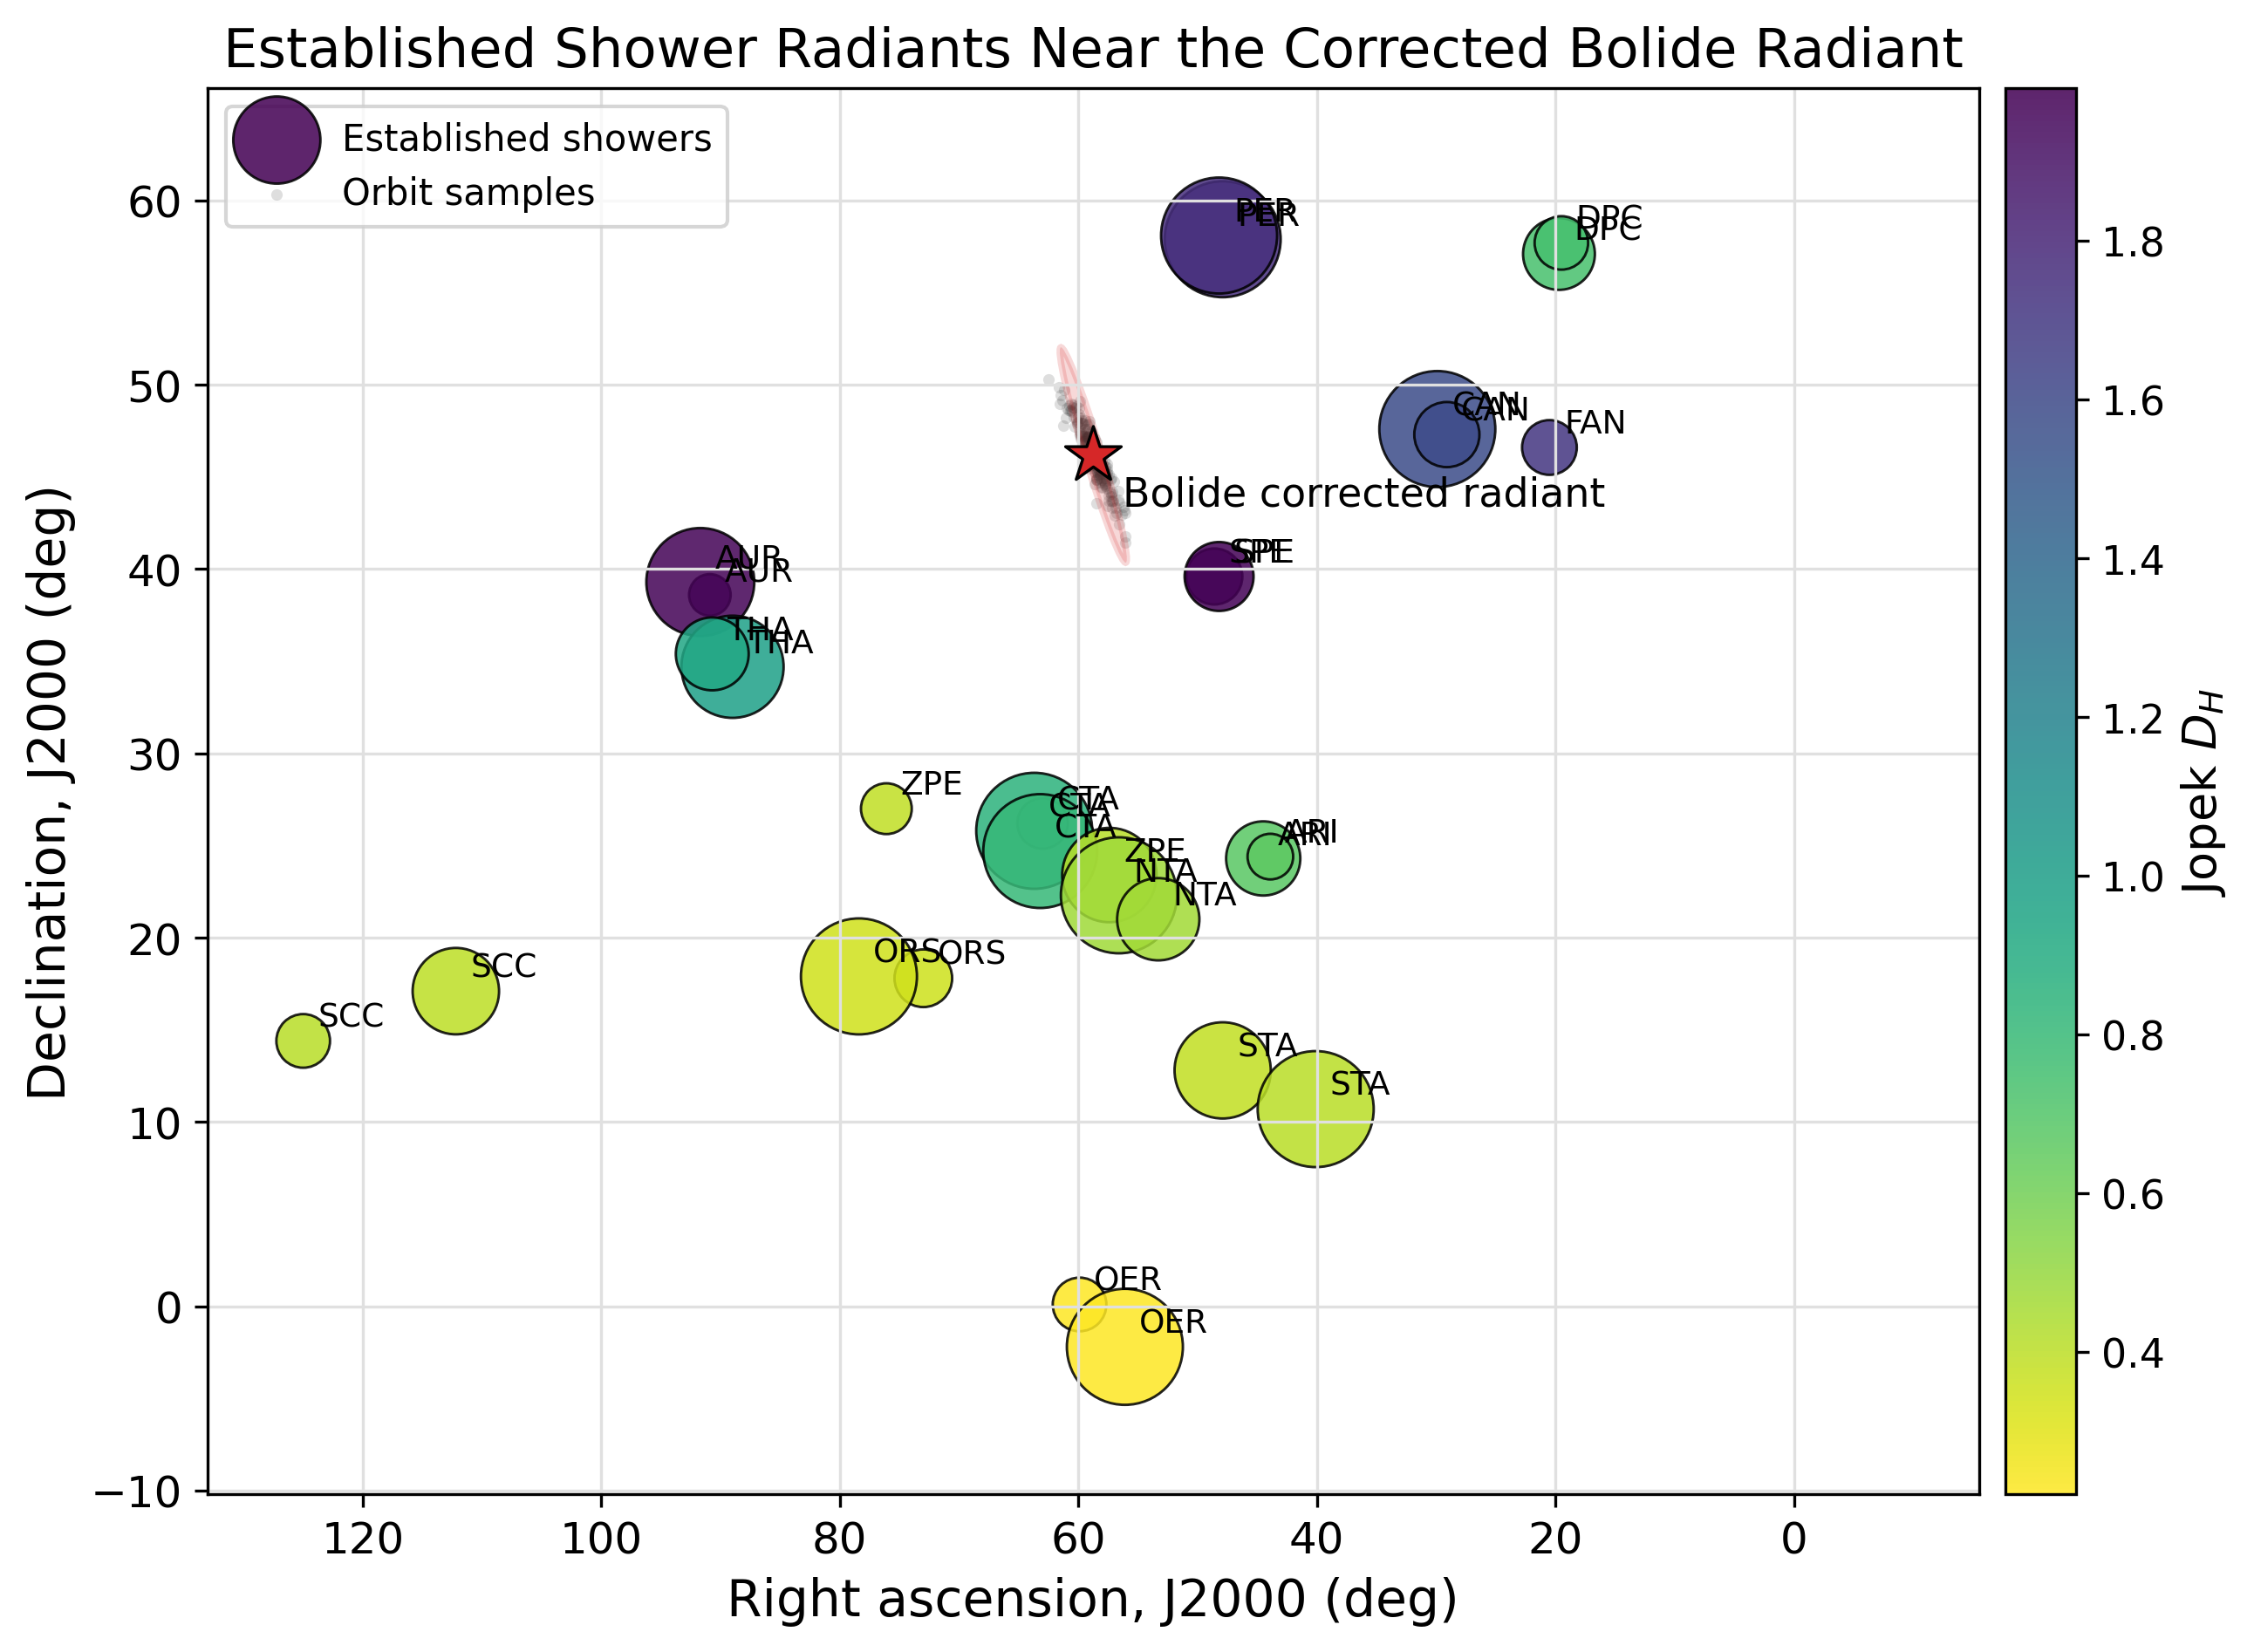
\includegraphics[width=0.92\linewidth]{figures/shower_radiant_comparison.png}
  \caption{Corrected bolide radiant compared with nearby established shower
  radiants from Jenniskens or Brown catalogue entries.  Red points show the
  2000 REBOUND-sampled zenithal-attraction-corrected bolide radiants, with
  red contours showing their sampled density and the star marking their mean.
  Shower marker area scales with catalogue member count, and color gives
  Jopek \(D_H\) orbital dissimilarity.}
  \figsource{plot_shower_radiants.py}
  \label{fig:shower-radiants}
\end{figure}

The closest NEA, comet, and established-shower entries are listed in
Table~\ref{tab:orbit-source}.  Agreement in \(D_H\) alone is not sufficient for
source identification: the radiant RA/Dec and geocentric speed provide
additional constraints, and the closest orbital-element match can still be a
poor radiant match.  Conversely, a nearby radiant without orbital-element
agreement is not by itself evidence for association.

The similar-body search should therefore be read as an orbital-neighbour
search rather than a parent-body identification.  The \(D_H\) function is a
hybrid form of the classical Southworth--Hawkins orbital dissimilarity
criterion \cite{southworth_hawkins_1963,jopek_1993}, and recent reviews
emphasize that \(D\)-criteria identify orbital similarity rather than genetic
association by themselves \cite{courtot_shober_vaubaillon_2026}.  Previous
radar stream tests also show that a single cutoff is not universal but depends
on the orbit distribution, inclination regime, measurement uncertainty, and
sporadic background \cite{galligan_2001,courtot_shober_vaubaillon_2026}.  In
the present catalogue comparison,
\(D_H \leq 0.15\) is used only as a practical flag for notable orbital
neighbours.  By this criterion the search finds several NEAs with similar
orbits, including 2024 XR16 with \(D_H=0.099\), but no comparable comet match:
the closest comet is P/2009 WX51 (Catalina) with \(D_H=0.300\).  No
established shower is similar.  The closest shower by \(D_H\), the
omicron-Eridanids, has \(D_H=0.224\) and a corrected-radiant separation of
about \(48^\circ\), making it a poor association despite being the nearest
listed shower in orbital-element space.

\section{Discussion}

\begin{itemize}
  \item \textbf{Radar methodology.}  The event demonstrates the value of
  retaining raw complex coded-CW voltage and reprocessing it with a
  range--Doppler matched-filter bank rather than relying only on routine
  meteor-radar detections.  The head echo is a high-Doppler feature and is
  easily masked by near-zero-Doppler trail/clutter power unless Doppler-gated
  and Doppler-whitened products are formed.  Storing the complex matched-filter
  output at the selected Doppler bin also preserves the information needed to
  revisit transmit AoD solutions.

  \item \textbf{Complementary head and trail constraints.}  The head echo
  provides timed bistatic range and Doppler measurements of the moving
  meteoroid, while the non-specular trail echoes provide spatial constraints
  on the line left behind in the atmosphere.  This separation is important
  physically: the trail plasma persists after passage and therefore constrains
  the path, not generally the instantaneous meteoroid time.  For the lowest
  trail echoes, however, the prompt and rapidly decaying behavior motivates the
  additional \(1\pm1\) s timing constraint used in the ballistic fit.
  A related physical caveat is that non-specular trail echoes are not
  necessarily produced at the instantaneous meteoroid head location.  They can
  arise from displaced plasma-trail scattering regions, so some vertical and
  geographic scatter is expected even with perfect interferometry.  The
  3 km coded-CW range resolution must also be included in this interpretation,
  because range quantization and interpolation uncertainty map into kilometre-
  scale position errors when combined with AoD constraints.

  \item \textbf{Low-altitude non-specular trail echoes.}  The fitted trail
  positions extend down to about 20 km altitude, far below the usual
  mesosphere/lower-thermosphere altitude range targeted by specular meteor
  radars.  Comparable multistatic fireball and re-entry studies generally
  emphasize trail/head-echo detections in the tens of kilometres above this
  level \cite{vierinen_2022_pajala,obenberger2026first,
  vierinen_2026_falcon9}.  If confirmed with additional quality control and
  external optical/GLM constraints, these low-altitude echoes are one of the
  most unusual radar signatures of the Cape Cod Bay event and may be related to
  strong fragmentation, dense plasma production, and/or favourable bistatic
  scattering geometry.

  \item \textbf{Orbit and source association.}  The current orbit solution is
  propagated from the ballistic head/trail covariance, so the plotted orbit and
  radiant uncertainties reflect the state uncertainty in the ballistic fit.
  The catalogue search finds several nearby NEA orbits but no similar
  established shower and no comparable comet match.  The \(D_H\) values should
  therefore be interpreted as an orbital-neighbour search rather than evidence
  for a specific parent body.

  \item \textbf{Sea-fall estimate.}  The radar-constrained ballistic path and
  the lowest trail positions place the late trajectory over Cape Cod Bay.  The
  nominal 10 cm dark-flight extrapolation produces a sea-level crossing in the
  bay, and sampling 1--100 cm fragments gives a broad impact-time and
  impact-position envelope.  The spread is dominated by unknown fragment size
  and post-fragmentation aerodynamics, not by the radar path near 30 km.

  \item \textbf{Relation to NASA public estimates.}  The radar solution is
  broadly consistent with the public NASA description of a northwest-to-
  southeast path and a meteorite fall into Cape Cod Bay.  However, the public
  estimates changed from an initial 40 mile, 75,000 mph, 300 ton TNT statement
  to a later 31 mile, 42,000 mph, 230 ton TNT statement
  \cite{afp_2026_new_england_meteor,ap_2026_new_england_meteor}.  The NASA
  size, mass, speed, altitude, and energy values should therefore be cited
  cautiously until a primary technical source is located; at present they are
  best treated as useful independent context rather than as fit constraints.
\end{itemize}

\section{Conclusions}

The Cape Cod Bay bolide was detected by a multistatic coded-CW meteor radar
system in both high-Doppler head echo and near-zero-Doppler non-specular trail
echo modes.  Range--Doppler matched filtering, Doppler whitening, and
multi-station bistatic fitting yield a steeply descending trajectory over the
Massachusetts coast.  Adding trail AoD plus bistatic-delay positions and a
simple ballistic drag model gives a physically motivated path that extends to
the lowest retained non-specular trail echoes and supports a likely sea fall
in Cape Cod Bay.

The inferred heliocentric orbit has finite but non-negligible uncertainty.
Within that uncertainty, the source-association search does not identify a
similar established meteor shower or cometary orbit.  Some NEA orbits are
nearby under the Jopek \(D_H\) criterion, but those similarities should be
treated as catalogue neighbours rather than parent-body identifications.

\section{Future Work}

Future analysis should focus on five items.  First, the GOES-19 GLM event,
group, and flash products should be obtained and compared directly with the
radar path and timing.  Second, infrasound and seismic waveform searches should
be performed to constrain the fragmentation timing and acoustic source region.
Third, the low-altitude non-specular trail solutions should be revisited with
stricter AoD ambiguity tests and, where possible, with station-by-station
coherence diagnostics.  Fourth, a fragmentation-aware dark-flight model should
replace the current fixed-density spherical-fragment sweep before any
meteorite-recovery guidance is attempted.  Finally, the NASA public estimate
of size, mass, speed, and energy should be traced to a primary technical source
or recalculated independently from optical/GLM/infrasound data.
